\documentclass[10pt,a4paper,english]{article}
\input premiamble
\input premiadata

\usepackage{amsmath,amsthm,amssymb}
\usepackage{babel}
\usepackage{graphicx}
\usepackage{color}

\newcommand{\ban}{\begin{eqnarray*}}
\newcommand{\ean}{\end{eqnarray*}}
\newcommand{\ba}{\begin{eqnarray}}
\newcommand{\ea}{\end{eqnarray}}

\begin{document}


\author{Marc BARTON-SMITH\footnote{ENPC, CERMICS, France} \quad Jos\'e da FONSECA\footnote{INRIA Rocquencourt, Projet Mathfi, France} \quad Marouen MESSAOUD\footnote{INRIA Rocquencourt, Projet Mathfi, France} \\ \quad Nicola MORENI\footnote{ENPC, CERMICS, France}}
\title{Libor Market Model}
\date{\today}
\maketitle
\thispagestyle{myheadings}
\tableofcontents

\vspace{10mm}




%%\section{Derivative products}

\section{Derivative products}



We note $B(t,T)$ the value of a zero coupon bond at time $t$ with maturity $T$.  

We suppose the following date structure $\lbrace T_n=T_0+n\tau ; n=1..M \rbrace $ 

the foward swap rate starting at date $T_s$ and ending at $T_M$ is given by 


\ban
S(t,T_s,T_M)=\frac{B(t,T_s)-B(t,T_M)}{\sum_{j=s+1}^{M}\tau B(t,T_j)}
\ean

the spot swap rate is $S(T_s,T_s,T_n)=S(T_s,T_M)$.

We note $L(t,T_i,\tau)$ the forward rate which set at time $T_i$ the cash flow received at time $T_i+\tau$. Arbitrage leads to  

\ba
1+\tau L(t,T_i,\tau)=\frac{B(t,T_i)}{B(t,T_{i+1})} 
\ea

spot libor rate is given by 

\ba
1+\tau L(T_i,T_i,\tau)=\frac{1}{B(T_i,T_{i+1})} 
\ea

remark: it is a simple rate.


Main products of interest for the libor Market Model

{\bf Caplet and floorlet}
suppose that  $t<T_M<T_{M+1}$

\begin{itemize}
\item we note $Cplt(t,T_M,K,\tau,N)$ the european caplet with  maturity $T_M$, strike $K$  on the spot libor rate $L(t,t,\tau)$ with  nominal value $N$ then at time $T_{M+1}=T_M+\tau$ the payoff is given by 
\ban
N \tau (L(T_M,T_M,\tau)-K)_+
\ean

\item we note $Flt(t,T_M,K,\tau,N)$ the european  floorlet  with maturity $T_M$, strike $K$  on the spot libor rate $L(t,t,\tau)$ with nominal value $N$ then at time $T_{M+1}=T_M+\tau$ the payoff is given by 

\ban
N \tau (K-L(T_M,T_M,\tau))_+
\ean
\end{itemize}

the cash flow at time $T_{M+1}=T_M+\tau$ is fixed at time $T_M$



{\bf Cap and floor} 
suppose that  $t=T_0<T_1<..<T_M$
\begin{itemize}
\item we note $Cap(t,T_s,T_M,K,\tau , N )$ the european  cap with maturity  $T_M$, strike $K$  on the spot rate $L(t,t,\tau)$ then at times $T_{s+1},...,T_M$ the option leads the cash flows  $N \tau (L(T_{s},T_{s},\tau)-K)_+, N \tau (L(T_{s+1},T_{s+1},\tau)-K)_+,.., N\tau (L(T_{M-1},T_{M-1},\tau)-K)_+$ ie 

\ban
\textrm{at $T_i$  cash flow } N \tau (L(T_{i-1},T_{i-1},\tau)-K)_+
\ean

\item we  note $Floor(t,T_s,T_M,K,\tau , N)$ the european floor with maturity $T_M$, strike $K$  on the spot libor rate $L(t,t,\tau)$ then at times $T_{s+1},...,T_M$ the option leads the cash flows  $N \tau (K-L(T_s,T_s,\tau))_+,N \tau (K-L(T_{s+1}1,T_{s+1},\tau))_+,..,N \tau (K-L(T_{M-1},T_{M-1},\tau))_+$ 

\ban
\textrm{at  $T_i$  cash flow } N \tau (K-L(T_{i-1},T_{i-1},\tau))_+
\ean

\end{itemize}

\begin{enumerate}
\item a cap is a portfolio of  caplets 
\ban
Cap(t,T_s,T_M,K,\tau, N )=\sum_{i=s}^{M-1}Cplt(t,T_i,K,\tau , N )
\ean
\item a floor is a portfolio of floorlets
\ban
Floor(t,T_s,T_M,K,\tau , N )=\sum_{i=s}^{M-1} Flt(t,T_i,K,\tau , N )
\ean
\end{enumerate}

{\bf Swaption} 
we suppose that  $t<T_0<T_1<..<T_M$ and we note $S(t,t,T_M)$ the swap rate with maturity $T_M$
\begin{itemize}
\item we note $Swpt(t,T_s,T_M,K,\tau,N)$ the european payer swaption with maturity $T_s=T$,  strike $K$ and nominal $N$  on the swap rate  $S(t,t,T_M)$   then at $T_s$ the exercise leads the cash flows:


\ban
\textrm{at $T_i$  cash flow } N \tau (S(T_s,T_s,T_M)-K)_+ \quad \textrm{for }i=s+1..M
\ean

\item we note $Swpt(t,T_s,T_M,K,\tau,N)$ the european receiver swaption with maturity $T_s=T$,  strike $K$ and nominal $N$  on the swap rate  $S(t,t,T_M)$   then at $T_s$ the exercise leads the cash flows:


\ban
\textrm{at $T_i$  cash flow } N \tau (S(T_s,T_s,T_M)-K)_+ \quad \textrm{for }i=s+1..M
\ean

\end{itemize}







%\section{Libor Market Model}


\section{Libor Market Model}


We suppose  $t \leq T_0 < T_1 <..<T_M $ with  $T_i=T_0+i \tau$ and  $T_{i+1}-T_i=\tau $ 
 

Recall that 

\ban
1+\tau L(t,T_i,\tau)=\frac{B(t,T_i)}{B(t,T_{i+1})} 
\ean

and

\ban
S(t,T_s,T_M)=\frac{B(t,T_s)-B(t,T_M)}{\sum_{j=s+1}^{M}\tau B(t,T_j)}
\ean

\ban
\frac{B(t,T_i)}{B(t,T_s)}=\prod_{j=s}^{i-1}\frac{1}{1+\tau L(t,T_j,\tau)}
\ean

as such the forward swap rate as a function of the forward rates is given by the relation

\ba
S(t,T_s,T_M)=\frac{1 - \prod_{j=s}^{M-1}\frac{1}{1+\tau L(t,T_j,\tau)} }{\sum_{j=s+1}^{M}\tau \prod_{k=s}^{j-1}\frac{1}{1+\tau L(t,T_k,\tau)}} \label{tswaptfor}
\ea

In the libor market model we suppose the following dynamic for the forward Libor rates


\ban
dL(t,T_i,\tau)=L(t,T_i,\tau)\gamma(t,T_i,\tau)dW^{Q^{T_{i+1}}}
\ean

where $\lbrace W^{Q^{T_{i+1}}}_t; t\geq 0 \rbrace$ is a $d$ dimensional brownian motion under the forward probability $Q^{T_{i+1}}$ associated with the numeraire $B(t,T_{i+1})$ and  $\gamma(t,T_i,\tau)$ is a deterministic function. 

Furthermore we know that 

\ban
d\left(\frac{B(t,T_i)}{B(t,T_{i+1})}\right)=\left( \frac{B(t,T_i)}{B(t,T_{i+1})} \right) (\sigma_B(t,T_i)-\sigma_B(t,T_{i+1}))dW^{Q^{T_{i+1}}}_t
\ean

where $\sigma_B(t,T)$ stands for the volatility of the zero coupon bond so from 

\ban
\frac{dL(t,T_i,\tau)}{L(t,T_i,\tau)}=\frac{1+\tau L(t,T_i,\tau)}{\tau L(t,T_i,\tau)}(\sigma_B(t,T_i)-\sigma_B(t,T_{i+1}))dW^{Q^{T_{i+1}}}_t
\ean

we get the relation

\ba
\frac{\gamma(t,T_i,\tau)\tau L(t,T_i,\tau)}{1+\tau L(t,T_i,\tau)}=\sigma_B(t,T_i)-\sigma_B(t,T_{i+1}) \label{volforvolzc}
\ea


this equation leads  from  (\ref{volforvolzc}) we have for  $j>i$

\ban
\sigma_B(t,T_j)-\sigma_B(t,T_i)=-\sum_{k=i}^{j-1}\frac{\gamma(t,T_k,\tau)\tau L(t,T_k,\tau)}{1+\tau L(t,T_k,\tau)}
\ean

it is well known that 

\ban
dW_t^{Q^{T_i}}+\sigma_B(t,T_i)dt=dW_t^{Q^{T_j}}+\sigma_B(t,T_j)dt
\ean

changing from zero coupon bond volatilities to forward rate volatilities we have for  $j>i$

\ban
dW_t^{Q^{T_i}}=dW_t^{Q^{T_j}}-\sum_{k=i}^{j-1}\frac{\gamma(t,T_k,\tau)\tau L(t,T_k,\tau)}{1+\tau L(t,T_k,\tau)}dt
\ean

\subsection{Pricing a caplet in the LMM framework}


Within the LMM the forward libor rate $L(t,T_i,\tau)$ follows the dynamic 

\ban
dL(t,T_i,\tau)=L(t,T_i,\tau)\gamma(t,T_i,\tau)dW^{Q^{T_{i+1}}}_t
\ean


suppose   $t<T_j<T_{j+1}$ and  $Cplt(t,T_j,K,\tau,N)$ a european  caplet with  maturity $T_j$,  strike $K$, nominal $N$  on the spot libor rate $L(t,t,\tau)$ then at time $T_{j+1}=T_j+\tau$ the cash flow is 

\ban
\tau (L(T_j,T_j,\tau)-K)_+N
\ean


\ban
Cplt(t,T_j,K,\tau,N)&=&E^Q_t\left[\frac{B(t)}{B(T_{j+1})}\tau (L(T_j,T_j,\tau)-K)_+N \right]\\
&=&E^{Q^{T_{j+1}}}_t\left[\frac{B(t,T_{j+1})}{B(T_{j+1},T_{j+1})}\tau (L(T_j,T_j,\tau)-K)_+N \right]\\
&=&B(t,T_{j+1}) N\tau E^{Q^{T_{j+1}}}_t\left[(L(T_j,T_j,\tau)-K)_+ \right]\\
&=& N \tau B(t,T_{j+1}) \left( L(t,T_{j},\tau)N(d_1)-KN(d_2)\right)
\ean

\ban
d_1&=&\frac{ln \frac{L(t,T_j,\tau)}{K} + \frac{1}{2}\int_t^{T_j}\gamma(u,T_j,\tau)^2du}{\sqrt{\int_t^{T_j}\gamma(u,T_j,\tau)^2 du}}\\
d_2&=&d_1 -\sqrt{\int_t^{T_j}\gamma(u,T_j,\tau)^2 du}
\ean


we get a formula consistent with market practice which quotes option through black volatility

\subsection{Pricing a swaption in the LMM framework}\label{DerPrdcts}

We briefly present the pricing of a swaption within the LMM framework and refer to \cite{braceGatarekMusiela}. Recall that 

\ban
Swpt(t,T_s,T_M,K,\tau)&=&\sum_{i=s+1}^ME^Q_t\left[ \frac{B(t)}{B(T_i)}\tau (S(T_s,T_s,T_M)-K)_+ \right]\\
&=&\tau \sum_{i=s+1}^MB(t,T_i)E^{Q^{T_i}}_t\left[L(T_s,T_{i-1},\tau){\bf 1}_{D}\right] \\
&-&\tau \sum_{i=s+1}^MB(t,T_i)E^{Q^{T_i}}_t\left[K{\bf 1}_{D}\right]
\ean

where

\ban
{\bf 1}_{D}&=&{\bf 1}_{\left( S(T_s,T_s,T_M)>K \right)}\\
&=&{\bf 1}_{\left( 1>B(T_s,T_M)+K\sum_{i=s+1}^MB(T_s,T_i)\right) }\\
&=&{\bf 1}_{\left( 1>\sum_{i=s+1}^Mc_iB(T_s,T_i)\right) }\\
&=&{\bf 1}_{\left( 1>\sum_{j=s+1}^Mc_j\prod_{k=0}^{j-1}\frac{1}{1+\tau L(T_s,T_j,\tau)} \right) } 
\ean


under  $Q^{T_i}$ we have  

\ban
dL(t,T_{i-1},\tau)=L(t,T_{i-1},\tau)\gamma(t,T_{i-1},\tau)dW^{Q^{T_{i}}}_t
\ean

for  $i>j+1$ 

\ban
\frac{dL(t,T_j,\tau)}{L(t,T_j,\tau)}=\gamma(t,T_j,\tau)dW^{Q^{T_i}}_t - \sum_{k=j+1}^{i-1}\frac{\tau L(t,T_k,\tau) \gamma(t,T_k,\tau) \gamma(t,T_j,\tau) }{1+\tau L(t,T_k,\tau)}dt
\ean

for  $j\geq i$ 

\ban
\frac{dL(t,T_j,\tau)}{L(t,T_j,\tau)}=\gamma(t,T_j,\tau)dW^{Q^{T_i}}_t +\sum_{k=i}^{j}\frac{\tau L(t,T_k,\tau)\gamma(t,T_k,\tau)\gamma(t,T_j,\tau)}{1+\tau L(t,T_k,\tau)}dt
\ean
 
\paragraph{Computing  $E^{Q^{T_i}}_t\left[L(T_s,T_{i-1},\tau){\bf 1}_{D}\right]$: }


Brace, Gatarek and Musiela  \cite{braceGatarekMusiela} propose to freeze the drift: under  $Q^{T_i}$ for  $i>j+1$ and $u \in [t \; T_s]$

\ban
\frac{dL(u,T_j,\tau)}{L(u,T_j,\tau)}=\gamma(u,T_j,\tau)dW^{Q^{T_i}}_u - \sum_{k=j+1}^{i-1}\frac{\tau L(\textcolor{red}{t},T_k,\tau) \gamma(u,T_k,\tau) \gamma(u,T_j,\tau) }{1+\tau L(\textcolor{red}{t},T_k,\tau)}du  
\ean

under  $Q^{T_i}$ for  $i\leq j$ and  $u \in [t \; T_s]$

\ban
\frac{dL(u,T_j,\tau)}{L(u,T_j,\tau)}=\gamma(u,T_j,\tau)dW^{Q^{T_i}}_u +\sum_{k=i}^{j}\frac{\tau L(\textcolor{red}{t},T_k,\tau)\gamma(u,T_k,\tau)\gamma(u,T_j,\tau)}{1+\tau L(\textcolor{red}{t},T_k,\tau)}dt
\ean


under this assumption the forward rates are lognormal


for $i>j+1$

\ban
L(T_s,T_j,\tau)&=&L(t,T_j,\tau)e^{\int_t^{T_s}\gamma(u,T_j,\tau)dW_u^{Q^{T_i}}-\frac{1}{2}\int_t^{T_s}\gamma(u,T_j,\tau)^2du}\\
& & e^{-\sum_{k=j+1}^{i-1}\frac{\tau L(t,T_k,\tau)}{1+\tau L(t,T_k,\tau)} \int_t^{T_s}\gamma(u,T_k,\tau) \gamma(u,T_j,\tau) du  }
\ean

for $j \geq i$

\ban
L(T_s,T_j,\tau)&=&L(t,T_j,\tau)e^{\int_t^{T_s}\gamma(u,T_j,\tau)dW_u^{Q^{T_i}}-\frac{1}{2}\int_t^{T_s}\gamma(u,T_j,\tau)^2du}\\
& & e^{+\sum_{k=i}^{j}\frac{\tau L(t,T_k,\tau)}{1+\tau L(t,T_k,\tau)}\int_t^{T_s} \gamma(u,T_k,\tau) \gamma(u,T_j,\tau) du  }
\ean

\newpage
we can write 

\ban
L(T_s,T_j,\tau)&=&L(t,T_j,\tau)e^{\int_t^{T_s}\gamma(u,T_j,\tau)dW_u^{Q^{T_i}}-\frac{1}{2}\int_t^{T_s}\gamma(u,T_j,\tau)^2du}\\
 &+& e^{\sum_{k=1}^{i-1}\frac{\tau L(t,T_k,\tau)}{1+\tau L(t,T_k,\tau)}\int_t^{T_s} \gamma(u,T_k,\tau) \gamma(u,T_j,\tau) du}
e^{- \sum_{k=1}^{j}\frac{\tau L(t,T_k,\tau)}{1+\tau L(t,T_k,\tau)}\int_t^{T_s} \gamma(u,T_k,\tau) \gamma(u,T_j,\tau) du  }
\ean




\ban
\xi_j^i&=&\int_t^{T_s}\gamma(u,T_j,\tau)dW_u^{Q^{T_i}}\\
\nu_{kj}&=&\int_t^{T_s} \gamma(u,T_k,\tau) \gamma(u,T_j,\tau) du \\
\beta_j^i&=&\sum_{k=1}^{i}\frac{\tau L(t,T_k,\tau)}{1+\tau L(t,T_k,\tau)}\int_t^{T_s} \gamma(u,T_k,\tau) \gamma(u,T_j,\tau) du\ean


\ban
L(T_s,T_j,\tau)&=&L(t,T_j,\tau)e^{\xi_j^i  -\frac{1}{2}\nu_{jj} + \beta_j^{i-1}-\beta_j^j  }
\ean



$\nu=(\nu_{kj})$ is variance covariance of the rates.

{\bf Rank one approximation}

There is a vector $\alpha=(\alpha_{s+1},\alpha_{s+2},..,\alpha_{M})^t$ with $\alpha_j\geq 0$ such that $\nu\sim\alpha \alpha^t $

then
 

\ban
\xi_j^i& \sim & \alpha_{j}X  \quad \textrm{with}  \quad X \quad {\cal N}(0,1)\\
\nu_{kj}& \sim & \alpha_{k}\alpha_{j} \\
\beta_j^i& \sim &\alpha_{j} \sum_{k=1}^{i}\frac{\tau L(t,T_k,\tau)}{1+\tau L(t,T_k,\tau)}\alpha_{k}\\
& \sim &\alpha_{j}d^i
\ean


\ban
L(T_s,T_j,\tau)&=&L(t,T_j,\tau)e^{\alpha_{j}X -\frac{1}{2}\alpha_{jj} + \alpha_j(d^{i-1}-d^j) }
\ean


\ban
&&E^{Q^{T_i}}_t\left[L(T_s,T_{i-1},\tau){\bf 1}_{D}\right]=\\
&&E^{Q^{T_i}}_t\left[L(t,T_{i-1},\tau)e^{ \alpha_{i-1}X -\frac{1}{2}\alpha_{i-1}\alpha_{i-1} } {\bf 1}_{\left( 1>\sum_{j=1}^Mc_j\prod_{k=0}^{j-1}\frac{1}{1+\tau L(t,T_k,\tau)} e^{\alpha_{k}X -\frac{1}{2}\alpha_{k}\alpha_k + \alpha_{k}(d^{i-1}-d^k)} \right)    }\right]
\ean

we note 

\ban
\phi_{i-1}(x)=\sum_{j=1}^Mc_j\prod_{k=0}^{j-1}\frac{1}{1+\tau L(t,T_k,\tau)} e^{\alpha_{k}x -\frac{1}{2}\alpha_{kk} + \alpha_{k}(d^{i-1}-d^k)}
\ean

recall that  $c_k\geq 0$ and $c_M > 1$ 

\ban
\lim_{x \rightarrow -\infty}\phi_{i-1}(x)&=&0\\
\lim_{x \rightarrow +\infty}\phi_{i-1}(x)&=&+\infty\\
\phi_{i-1}'(x)&>&0 
\ean  

so there is a unique $\bar x_{i-1}$ such that $\phi_{i-1}(\bar x_{i-1})=1$, finally the expectation is given by  

\ban
E^{Q^{T_i}}_t\left[L(T,T_{i-1},\tau){\bf 1}_{D}\right]=\int_{\bar x_{i-1}}^{+ \infty} L(t,T_{i-1},\tau)e^{\alpha_{i-1}x -\frac{1}{2}\alpha_{i-1}\alpha_{i-1}} \frac{1}{\sqrt {2\pi}}e^{-\frac{x^2}{2}}dx
\ean

and we have $\bar x_{i}=\bar x_{i-1}+d^{i-1}-d^{i}$

It is possible to use a rank k approximation, see Brace \cite{brace1}.


\paragraph{ The spot measure}

In  the HJM framework, where interest rates are continuously coumpounded,  one usually uses the cash as risk free asset which follows the dynamic

\ban
dB(t)=B(t)r(t)dt
\ean

In the LMM framework we deal with simple interest rates as such it is possible to define the discret tenor bank account noted $B_d(t)$ as follow:


$\eta(t)$ such that  $\eta(t)=n $ if $t \in [T_{n-1} \; T_{n}[$

\ban
B_d(0)&=&1\\
B_d(t)&=&\prod_{j=0}^{\eta(t)}(1+\tau L(T_j,T_j,\tau))B(t,T_{\eta(t)})
\ean

which is an asset with unit value at time $t=0$ and discretly compounded in the spot rates

using $B_d(t)$ as numeraire we can define the ``spot libor measure'' $Q^d$ under which  $L(t,T_i,\tau)$ follows the dynamic

\ban
\frac{dL(t,T_i,\tau)}{L(t,T_i,\tau)}= \sum_{k=\eta(t)}^{i}\frac{\tau L(t,T_k,\tau)\gamma(t,T_k,\tau)\gamma(t,T_i,\tau)}{1+\tau L(t,T_k,\tau)}dt + \gamma(t,T_i,\tau)dW^{Q^d}_t
\ean


\paragraph{ Pricing under $Q^d$}: the value at time $t=0$ of a security paying $\xi$ at $T_n$ is given by

\ban
\pi(0)=E^{Q^d}\left[ \frac{B^d(0)}{B^d(T_n)}\xi \right]
\ean

Remark: suppose $\xi=1$ then $\pi(0)=B(0,T_n)$

\ban
B(0,T_n)=E^{Q^d}\left[ \prod_{i=0}^{n-1}\frac{1}{(1+\tau L(T_i,T_i,\tau))} \right]
\ean

one should recover bond values from the forwards.


% \section{Bushy Tree Technique}

%\newcommand{\winlin}{\backslash}
\newcommand{\winlin}{/}
\section{Bushy Tree Technique}
The bushy technique consists in using a non-recombining tree to estimate the evolution of the libor vector needed to price a fixed income derivative(Swaption, Cap, Floor, Bermudean Swaption). The feature of the tree method is clear when we need to compute American contract. Actually, in this case we need to compare between the exercise and the continuation strategies, and in order to compute the continuation value we must compute a conditional expectation for each realization of the libor vector, and here a tree method seems to be the easiest to establish.\\
The Libor Market Model is path dependent model, this appears in the drift, then we cannot use recombining tree methods. The disadvantage is that the number of nodes explodes with the number of time step and since we must enlarge the time step number to make the discontinuous process converge to the continuous one we are very quickly limited by the calculation time and by the finite memory size in the PC. This study is based on the \cite{Jackel} and \cite{TANGLANGE}. In the first the author gives a method to establish the transition matrix and also proposes a recursive algorithm to construct the Libor tree in order to compute the price. In the second article the authors present an non exploding bushy tree technique. It consists in choosing at a time step some number of nodes form which the tree continues diffusing and interpolate to get the value on the others.

\subsection{Optimal simplex alignment}
A tree is defined by its transition matrix which gives the probability of the underlying to move from one realization at time t to another one at time t+dt. We must also define the realizations on the tree or more simply, we must know the possible realizations that the underlying can do form one node. For example in the trinomial tree we must choose or compute the (u,m,d) parameters. In many cases methods are proposed to fit the first and second moment of the underlying. It is much careful to consider directly the gaussian variable since it is the source of randomness. For example  :

\begin{math}
S^{(1)} = \left(
\begin{array}{c}
			-1 \\
      1 
\end{array}
\right)
\end{math}

\begin{math}
S^{(2)} = \left(
\begin{array}{c c}
			-\sqrt{\frac{3}{2}} & -\sqrt{\frac{1}{2}} \\
      \sqrt{\frac{3}{2}} & -\sqrt{\frac{1}{2}} \\
      0 & \sqrt{2} \\ 
\end{array}
\right)\\
\end{math}
For a m dimension general case we define the simplex $S^{(m)}$ as :
\begin{math}
S^{(m)}_{ij} = \left\{
\begin{array}{c c}
			-\sqrt{\frac{m+1}{(j+1)j}} & for\  j\geq i \\
			\sqrt{\frac{m+1}{(j+1)j}} & for\  j= i-1 \\
			0 & for\  j< i-1
\end{array}
\right.
\end{math}
Given the uncorrelated covariance matrix $\overline{A}$ after a Cholesky decomposition we can define the branching matrix
$$\overline{B}=\overline{A}.S^{T}$$
and construct the bushy tree of the libor.
the recursive algorithm for a European swaption is called by Recurse(0) :
\small{
\begin{verbatim}
double Recurse(long h){
	long i,k;
	double tmp=0;
	double ProdLibor=1,SumLibor=0.0,SwapRate,Bsi=1,SumBsi=0.0,res=0.0;
	if (h==NSteps){
		for(i=0;i<NRates;i++)
		{
			ProdLibor*=(1+EvolvedFra[h][i]*period);
			SumLibor += period/ProdLibor;
		}
		SwapRate=(1-(1/ProdLibor))/(SumLibor);
		
		for(i=0;i<NRates;i++)
		{
			Bsi*=1.0/(1+period*EvolvedFra[h][i]);
			SumBsi += Bsi;
		}
		res = (B0*SumBsi*period*MAX(type*(SwapRate-strike),0.0));
		return res;
	}
	
	for (i=0;i<NRates;i++){ // Calculate the drift for all rates and store them.
		mu_dT[h][i] = 0.;
		for (k=NumeraireIndex;k<=i;k++)
			mu_dT[h][i] += C[h][i][k] * EvolvedFra[h][k] * period / ( 1. + EvolvedFra[h][k] * (period) );
	}
	
	for (k=0;k<NBranches;k++){ // Loop over all branches.
		for (i=0;i<NRates;i++){
			EvolvedFra[h+1][i] = EvolvedFra[h][i] * exp( mu_dT[h][i]*(Tau[h+1]-Tau[h]) +
																											 LogShiftOfBranch[h][k][i] );
		}
		tmp += Recurse(h+1); // Sum up the results from all of the branches.
	}
	return tmp/NBranches;
}

\end{verbatim}
}
The author proposes also a method to rotate the branching matrix in order to fill the space in a best way and take benefit out of the use of more branches.
$ S^{m} \stackrel{R^m}{\rightarrow}S^{'m}$ such that
\begin{eqnarray}\label{rotate}
 S^{'(m)}_{i j}=-S^{'(m)}_{m+2-i j}\ for \ m \ even \ and \ j=1\ldots \frac{m}{2}\\
 S^{'(m)}_{i j}=-S^{'(m)}_{m+2-i j}\ for \ m \ odd \ and \ j=1\ldots \frac{m+1}{2}
\end{eqnarray}
This can be done using some optimization technique. In the space $\mathbb{R^{m}}$ a rotation can be construct by a composition of $\frac{m(m-1)}{2}$ rotation in a each hyperplane. Then we can write 
\begin{equation}
R^m = R^{m}(\theta_1) \ldots R^{m}(\theta_{\frac{m(m-1)}{2} } )
\end{equation}

The problem is to find the $\frac{m(m-1)}{2}$ unknown variables $\theta$ in order to get a rotated matrix $S$ that solve the system (\ref{rotate}). We used a MCO criteria that we minimized using a newton method based on BFGS algorithm. This procedure can be done before calling the pricing routine and we do it only one time for all the tree and for all the product to price. We recall that in our approach we construct a tree for the gaussian random variable and this is independent from the volatility structure and from the other parameters of the BGM model, then we plug it in our model to get a tree that corresponds to our specific model.
\subsection{Remarks}
\label{sec:Remarks}
The non recombining tree method is huge time consuming and the time of calculation explodes very fast with the number of time step that leading to maturity. This method can not be used to price a non path dependent product since the Monte-Carlo method is much simpler to implement and is very fast. For path dependent product the non recombining tree can give an indicative price and is suitable for these products but it falls down with the limitation of the number of time step.
For the non exploding bushy tree we can price with more number of time step. The only limitation is the interpolation on the nodes where the tree does not continue diffusing. The problem is that this method is very sensitive to the moneyness of the product. Actually suppose that we have a vector of nodes with a their real corresponding values
\begin{math}
\left[
\begin{array}{c}
			5\\
      4\\
      0\\ 
      0\\
      0\\
      0\\
\end{array}
\right]\\
\end{math}
on a uniform distributed tree the average is 1.5. On a non exploding bushy tree suppose that we used only the first and the last nodes to continue the expansion of the tree and interpolate on the 4 interior nodes, we get
\begin{math}
\left[
\begin{array}{c}
			5\\
      4\\
      3\\ 
      2\\
      1\\
      0\\
\end{array}
\right]\\
\end{math}
and the average is 2.5 which is much bigger than the real value. This is only an illustrative example, but this is what it happens on the non exploding bushy tree. If our product is deep in the money we get a quite reasonable error. If the product is out of the money the error is too big and we can not accept this method. In the figures (\ref{fig:SwaptionPayeur75}) , (\ref{fig:SwaptionPayeur25}) ,(\ref{fig:SwaptionReceveur75}),(\ref{fig:SwaptionReceveur25}) the sign $+$ means with and the sign $-$ means without. The figure (\ref{fig:SwaptionReceveurTime25}) shows the exponential growth of the computation time with the bushy tree and with the non exploding bushy tree. We see that we can use the bushy tree technique up to 20 time steps and we can go further up to 30 steps using the non exploding bushy tree. The problem is the using a tree to model a diffusion we must use a large number of time step to get the convergence of our scheme to the continuous model. With the bushy tree technique this can not be fulfill since we are limited by the exponential growth of the computation time. Figures (\ref{fig:SwaptionPayeur25_6}),(\ref{fig:SwaptionReceveur25_6}) shows the impact of rotating the simplex on the Bushy tree techniques. This is similar to using a less discrepancy random generator in the Quasi Monte-Carlo approach. Also here, rotating the simplex is efficient when we deal with large dimension problem and this is shown on the following figures.
\begin{figure}[htbp]
	\centering
		\includegraphics[width=0.60\textwidth,angle=-90]{figures\winlin SwaptionPayeur75.eps}
	\caption{SwaptionPayeur75}
	\label{fig:SwaptionPayeur75}
\end{figure}
\begin{figure}[htbp]
	\centering
		\includegraphics[width=0.60\textwidth,angle=-90]{figures\winlin SwaptionReceveur75.eps}
	\caption{SwaptionReceveur75}
	\label{fig:SwaptionReceveur75}
\end{figure}
\begin{figure}[htbp]
	\centering
		\includegraphics[width=0.60\textwidth,angle=-90]{figures\winlin SwaptionPayeur25.eps}
	\caption{SwaptionPayeur25}
	\label{fig:SwaptionPayeur25}
\end{figure}
\begin{figure}[htbp]
	\centering
		\includegraphics[width=0.60\textwidth,angle=-90]{figures\winlin SwaptionReceveur25.eps}
	\caption{SwaptionReceveur25}
	\label{fig:SwaptionReceveur25}
\end{figure}
\begin{figure}[htbp]
	\centering
		\includegraphics[width=0.60\textwidth,angle=-90]{figures\winlin SwaptionPayeur25_6.eps}
	\caption{SwaptionReceveur25,6 libor}
	\label{fig:SwaptionPayeur25_6}
\end{figure}
\begin{figure}[htbp]
	\centering
		\includegraphics[width=0.60\textwidth,angle=-90]{figures\winlin SwaptionReceveur25_6.eps}
	\caption{SwaptionReceveur25,6libor}
	\label{fig:SwaptionReceveur25_6}
\end{figure}
\begin{figure}[htbp]
	\centering
		\includegraphics[width=0.60\textwidth,angle=-90]{figures\winlin SwaptionReceveurTime25.eps}
	\caption{SwaptionReceveur25}
	\label{fig:SwaptionReceveurTime25}
\end{figure}






%\section{Bermudan swaption pricing in the Libor Market Model}




\section{Bermudan swaption pricing in the Libor Market Model}

While in section \ref{DerPrdcts}  we introduced the most common \emph{vanilla} 
interest rate products, namely Caps, Floors and European Swaptions, the aim of the present 
one is to describe some \emph{exotic} products which undergo the name of Bermudan Swaptions.\\ 

Let us consider as before a tenor structure $T_0,\ldots,T_M$ and define an \emph{ending date} $T_e$ and a \emph{starting date} $T_s$ such that $T_0\leq T_s\leq T_e\leq T_M$.
There are (at least) two possibility of setting up a Bermudan Swaption agreement: one with  \emph{fixed-maturity} and one with \emph{fixed-lenght}. A fixed-maturity  Bermudan Swaption is an agreement which gives the owner the right of chosing, at each $T_i$ with $s\leq i\leq e$,  whether to enter or not into an European Swaption over $[T_i,T_e]$, while a Bermudan Swaption with a fixed lenght of $m\in\mathbb{N}$ tenor periods, will give the owner the right to enter into an European Swaption over $[T_i,T_{i+m}]$. From now on, we will restrict to the case of fixed-maturity Bermudan Swaptions, extension to  fixed-lenght ones being straightforward\footnote{See for instance \cite{Pedersen99} for details.}.\\

Entering a payer  $[T_i,T_e]$-European Swaption with strike $K$ and nominal value $\mathcal{N}$,   means to be payed at time  $T_i$ the quantity\footnote{For simplicity of notation, we omit functional dependence on $K$ and $\mathcal{N}$, considered as fixed throughout the following.} 
\ba
Swpt(T_i;T_i,T_e) \doteq \left(\sum_{j=i+1}^{e-1}\mathcal{N}\tau B(T_j,T_e)\right) (S(T_i,T_i,T_e)-K)_+
\ea   
where $S(T_i,T_i,T_e)$ is the swap rate corresponding to the chosen swap agreement.\\
Thus, price at time $t<T_s$ of a  Bermudan swaption with starting date $T_s$ and fixed-maturity $T_e$, is given, under the measure $\mathbb{Q}^Y$ corresponding to a given price process $Y$ as numeraire, by 
\ba\label{optimalstopping}
U(t)=\sup_{\bar \tau\in\mathcal{T}^{s,e-1}}E^Y_{t}\left[\frac{Y(t)}{Y(\bar \tau)}Swpt(\bar \tau;\bar \tau,T_e)\right],
\ea  
where $\mathcal{T}^{s,e-1}$ is the set of stopping times $\bar \tau$ taking values in $\{T_s,\ldots,T_{e-1}\}$.
Standard theory of optimal stopping time \cite{LambLap} ensures us that $U(0)$ is the solution of the following  dynamic programming problem:
\begin{equation}\label{dynamicprogramming}\left\{\begin{aligned}
U_{e-1}&= Swpt(T_{e-1};T_{e-1},T_e)\\
U_i\:&=\max\left\{Swpt(T_{i};T_{i},T_e),E^Y_{T_i} \left[\frac{Y(T_i)}{Y(T_{i+1})}U_{i+1}\right]\right\}, {\forall\,i=s,\ldots,e-2}\\
U_0\:&=E^Y_{T_0} \left[\frac{U_s}{Y(T_s)}\right]
\end{aligned}\right.\end{equation}
where for simplicity of notation we set $U(T_i)=U_i$. The dynamic programming formulation is clearly less synthetic than the optimal stopping time one but is of easier implementation. \\
\subsection{Monte Carlo Pricing of Bermudan Swaptions with the Longstaff-Schwartz Algorithm}
Due to the necessity of comparing at each time $T_i$ the exercise value $Swpt(T_{i};T_{i},T_e)$ to the continuation value  $V_i\doteq E^Y_{T_i} \left[\frac{Y(T_i)}{Y(T_{i+1})}U_{i+1}\right]$, pricing of early excercise derivatives on high dimensional underlying (here the forward rates) is usually performed \emph{via} Monte Carlo simulations or by means of trees methods. In Premia we implement the MC algorithm which was firstly  introduced by Longstaff and Schwartz in 2001 and which is based on a least squares approach. As this algorithm is widely described in the PremiaDoc section devoted to Monte Carlo methods for asset derivatives, here we will only report main ideas for self-consistency.\\
Let us take a look to equation (\ref{dynamicprogramming}): in order to price a Bermudan Swaption, it is clear that we must be able to evaluate continuation values, a task which a priori is nor easy nor straightforward. However, by definition of conditional expectation, each continuation value $V_i$ can be seen  as the best $L^2$-approximation of the discounted $T_{i+1}$ price $Y(T_i)U_{i+1}/Y(T_{i+1})$ among the $\mathcal{F}_{T_i}$-measurable random variables. Thus,  following the authors, we choose an  $\mathcal{F}$-adapted  and square integrable stochastic process $X(t)$ together with a set of basis functions $\underline{e}=(e_1,\ldots,e_m)$ such that $E[e_i^2(X(t))]<\infty$ for all $t\leq T_e$ and we  set
\begin{equation}\label{leastsquares}\begin{aligned}
V_i&\approx \underline{a}_i\cdot \underline{e}(X(T_i))\\
\underline{a}_i&=\mathrm{arg}\min_{\underline{a}\in\mathbb{R}^M}E\left[\frac{Y(T_i)}{Y(T_{i+1})}U_{i+1}-\underline{a}\cdot \underline{e}(X(T_i))\right]^2.
\end{aligned}\end{equation} 
In other words, for all $i=s,\ldots,e-1$  we find the best approximation of $$Y(T_i)U_{i+1}/Y(T_{i+1})$$ in the $m$-dimensional subset of $L^2$ spanned by $\{e_1(X(T_i),\ldots,e_m(X(T_i))\}$. 
The goodness of such an approximation will rely on the \emph{``explanatory power''} of $X$ and on the choice of the basis functions. The Longstaff and Schwartz algorithm is then based on finding an approximated solution to the least squares problem (\ref{leastsquares}) by   considering $N$ independent samples of the forward rates stochastic process $L(t)=\{L(t,T_0,\tau),\ldots,L(t,T_{e-1},\tau)\}$ and of the \emph{explanatory variable} $X(t)$. It is then natural to approximate regression coefficients $\underline{a}_i$ by  
\ba\label{MCleastsquares}
\underline{a}_i\approx\underline{a}^N_i=\mathrm{arg}\min_{\underline{a}\in\mathbb{R}^M}\frac{1}{N}\sum_{n=1}^{N}\left[\frac{B^{(n)}(T_i)}{B^{(n)}(T_{i+1})}U^{(n)}_{i+1}-\underline{a}\cdot \underline{e}(X^{(n)}(T_i))\right]^2
\ea
where the superscript $^{(n)}$ stand for the $n$-th Monte Carlo call.
Finally, the dynamic programming problem (\ref{dynamicprogramming}) rewrites,
\begin{equation}\label{approxdynamicprogramming}\left\{\begin{aligned}
U^{N,(n)}_{e-1}&= Swpt^{(n)}(T_{e-1};T_{e-1},T_e)\\
U^{N,(n)}_i\:&=\max\left\{Swpt^{(n)}(T_{i};T_{i},T_e),\underline{a}^N_i\cdot \underline{e}(X^{(n)}(T_i))\right\}, {\forall\,i=s,\ldots,e-2}\\
U^N_0\:&=\frac{1}{N}\sum_{n=1}^{N}\left[\frac{U^{(n)}_s}{B^{(n)}(T_s)}\right]
\end{aligned}\right.\end{equation} 
Cl\'ement, Lamberton and Protter \cite{CLProtter} have proved convergence of such an algorithm to the original problem when $N$ and $m$ go to $+\infty$. In particular, when $N\rightarrow\infty$, a central limit theorem holds.\\
\subsection{Premia Implementation}
Implementing the Longstaff ans Schwartz algorithm, require the choice of a set of basis functions and of an explanatory variable. \\

Concerning the basis functions, Premia algorithm  allow for two options: a canonical  polynomial basis and an Hermite polynomial basis. At each timestep $T_i$, optimal coefficients $\underline{a}^N_i$, are found by regressing the $B^{(n)}(T_i)U^{(n)}_{i+1}/B^{(n)}(T_{i+1})$ over the $X^{(n)}(T_i)$. Moreover, for early steps of backward dynamic programming (regression for $T_{e-2}, T_{e-3},\ldots$) the price will not be very different from excercice value. With our algorithm it is thus possible to include the early excercise value in the regression basis, that is to set for the first basis function $e_1(X^{(n)}(T_i))=Swpt^{(n)}(T_{i};T_{i},T_e)$ for all $i$ greater than a given $\bar{i}$.\\ 

On the other side, the choice of an explicatory variable is more tricky and constrained by the necessity of keeping $m$ quite small  in order to make regression fast. Let us recall that the swap rate $S(T_i,T_i,T_e)$ is indeed a function of $L(T_i,T_i,\tau),\ldots,L(T_i,T_{e-1},\tau)$ and then the more natural explanatory variable would be the Libor state vector $L(t)$. However, imagine to consider a Bermudan swaptions with $\tau=0.5$ years, $T_s=3.0$ yars, $T_e=8.0$ years. Following above reasoning, we would need two Libors for regressing at time $T_{e-2}$ but we would need nine libors to regress at time $T_s$. Thus, for maturities close to $T_s$ we must have $m\approx 10$ to take into account all relevant Libors. Whenever considering long maturity swaptions, things get even worse. That is why Pieterz et al. \cite{Pelsser03} suggest to regress directly on the Notional Paying Value (NPV) $Swpt(\cdot,\cdot,T_e)$ while Pedersen \cite{Pedersen99} do test regression on the Numeraire, the fixed leg value $K\left(\sum_{j=i+1}^{e-1}\mathcal{N}\tau B(T_j,T_e)\right)$ and the prices of some European options embedded in the Bermudan contract. Pedersen concludes that the European prices are not relevant and that a quadratic function in the Numeraire and in the fixed leg value is accurate enough.\\

Premia users can set the explanatory variable to be 
\begin{itemize}
\item the notional paying value
\item the underlying Brownian motion
\item the Numeraire.
\end{itemize}
In table \ref{PremiavsPelsser} we report Premia pricing results and compare them to the ones obtained by Pietersz. et al. \cite{Pelsser03} with a Longstaff and Schwartz algorithm and their drift approximation method. In particular, we take a 1-Factor model with flat volatility (15\%) and initial forward rate values (5\%); the tenor $\tau$ is 0.5 years and the SDE is discretized with 10 timesteps for each tenor period. We price At-The-Money  Bermudan swaptions for various choices of starting and ending times $T_s$ and $T_e$ and  changing the explanatory variable (Brownian, NPV, Numeraire). Regression basis is four dimensional ($m=4$) and we used 10000 Monte Carlo calls.\\

\underline{R\small{EMARK}}  We strongly reccomend to include NPV  in regression basis when regressing onto the Brownian motion or the Numeraire, expecially for short lenght swaption, in which the difference between the european and the bermudan contract is small. On the other side, when regressing on the NVP, take care NOT to include the payoff into regression\footnote{It is sufficient to set $T_{\bar i}=T_{e-1}$.}  because it is likely to waste the performance of regression (Cholesky routine used for regression could return errors). For instance, regressing on the Numeraire, a choice $T_{\bar i}=5$ years is good enough either for a swaption with $(T_s,T_e)=(5,8)$ and for a $(1,8)$ swaption. When the lenght of the longest swaption $(T_s,T_e)$ is short, regression on Brownian motion seems to be more stable with respect to changes in   $T_{\bar i}$ than regression on the Numeraire.
\begin{table}[h!]\label{PremiavsPelsser}
\begin{tabular}{cc}
\hline
Pietersz et al. & Premia\\ 
\hline
\begin{tabular}{cccc}
$[T_s,T_e]$& Drift & L-S & Std\\
           &Approx &     & Err\\
\hline
1,2 &29.40  &28.85 &0.42\\  
1,3 &64.33  &62.78 &0.83\\  
1,4 &101.66 &101.51 &1.29\\  
3,4 &44.09  &43.59 &0.70\\  
%1,5 &141.22 &137.95 &1.68\\  
%3,5 &89.25  &86.75 &1.34\\  
1,6 &182.16 &179.48 &2.22\\  
3,6 &134.88 &136.43 &2.01\\  
5,6 &50.93  &50.79  &0.86\\  
%1,7 &224.40 &221.38 &2.61\\  
%3,7 &181.20 &177.11 &2.53\\  
%5,7 &101.84 &100.59 &1.64\\  
1,8 &266.63 &266.35 &3.15\\  
3,8 &226.55 &226.94 &3.14\\  
5,8 &151.23 &151.13 &2.38\\  
7,8 &54.20  &53.70 &0.96\\ 
\end{tabular}&
\begin{tabular}{ccc}
Brown.&Numer.&NPV\\&&\\
\hline
29,36&28,91&29,35\\
64,66&63,61&64,75\\
102,98&102,36&103,14\\
43,74&43,70&43,74\\
185.65&184,59&185,67\\
134,84& 132,40&134.96\\
49,66& 49,65& 49,66\\
264,00& 262,11&263,83\\
223.85& 219,54&223,94\\
148.07& 148.10&148,13\\
52.50&52.48 &52,49\\
\end{tabular}\\
\hline
\end{tabular}
\caption{Fixed-maturity Bermudan Swaptions prices for different starting and ending time. Pietersz, Pelsser and von Mortengel \cite{Pelsser03} Drift Approximation and Longstaff-Schwartz 1 Factor results compared to Premia 1-factor Longstaff-Schwartz with different choices for the explanatory variable.}
\end{table}


\subsection{List Of Inputs}
Inputs required by the algorithm are
\begin{itemize}
\item \emph{double} the tenor $\tau$ (in yrs) 
\item \emph{double} the starting date $T_s$, called ``swaption maturity'' (yrs)
\item \emph{double} the ending date $T_e$, called ``swap maturity'' (yrs)
\item \emph{int} the number of maturities (that is $T_e/\tau$)
\item \emph{double} the payoff as regressor $T_{\bar i}$: the time  after which regression will
include the NPV in the basis  
\item \emph{char*} the pricing measure. Numeraire can be either the Jamshidian 1997's roll-over money account
$J(T_i)=1/(\prod_{l=0}^{i-1}B(T_i,T_{i+1}))$ (spot measure) or the bond $B(\cdot,T_e)$ (terminal forward measure).
\item \emph{char*} the explanatory variable: Numeraire, NPV or Brownian Motion
\item  \emph{long} the number of Monte Carlo calls for pricing and regression
\item \emph{char*} the regression basis: canonical or Hermite polynomials
\item  \emph{int} the dimension $m$ of the regression basis $\underline e(\cdot)$
\item  \emph{int} the number of step to be used for SDE discretization over $[T_i,T_{i+1}]$
\item \emph{double} the number of factors
\item \emph{double} the strike $K$   
\end{itemize}

See ``lmm\_bermudatest.c'' for an example.


\subsection{Programming interface}


\subsubsection{C API of the pricer}

We define a simpler interface to the bermudan swaption pricer as follow:

\small{
\begin{verbatim}
double lmm_swaption_payer_bermudan_LS_pricer(tenor ,numberTimeStep, 
                 numFac, swaptionMat, swapMat, payoff_as_Regressor, numberMCPaths, 
                 Regr_Basis_Dimension, basis_name , measure_name , Explanatory , K)
\end{verbatim}
}

Arguments description:
\begin{itemize}
\item $tenor$ is the period in years of the rate (usually 3 or 6 months); type:double 
\item $numberTimeStep$ number of time steps in the euler scheme; type:int 
\item $numFac$ is the number of factors max 2; type: int
\item $swaptionMat$ is the swaption maturity in years; type: double
\item $swapMat$ is the swap maturity in years ; type: double 
\item $numberMCPaths$ number of monte carlo paths; type:long
\item $payoff\_as\_Regressor$ in (years) maturity after which payoff is included in regression
\item $Regr\_Basis\_Dimension$ finite-dimensional approximation of $L^2$ ; type: int
\item $basis\_name$ basis name; type: char*
\item $measure\_name$ measure name: type: char*
\item $Explanatory$ Explanatory variable for regression B=Brownian, S=Nominal Swap Paying Value, N=Numeraire;
\item $K$ strike; type:double
\end{itemize}

{\bf Remarks:}
\begin{enumerate}
\item To price a caplet just call the function with $swapMat=swaptionMat+tenor$
\item $swapMat$ must be equal to $k*tenor$ with $k$ an integer
\item $swaptionMat$ must be equal to $k*tenor$ with $k$ an integer
\item $payoff\_as\_Regressor$ must be equal to $k*tenor$ with $k$ an integer
\end{enumerate}

\subsubsection{calling the bermudan swaption pricer from a C program}

\small{

\begin{verbatim}
************************************************
 *   Bermudean Swaptions Pricer             
 *
 *   -Spot Probability Measure (Numeraire=Roll-Over Bond)
 *   -Possibility to include Martingale Discretization
 *   -Bermudean with fixed ending date.
 *   Nicola Moreni, August 2004 
 *
 ****************************************************/ 
 

#include<stdio.h>

#include"lmm_header.h"
#include"lmm_volatility.h"
#include"lmm_libor.h"
#include"lmm_random_generator.h"
#include"lmm_products.h"
#include"lmm_numerical.h"
#include"lmm_zero_bond.h"
#include"lmm_bermudaprice.h"

/*REMINDER:
-lmm_header.h contains structures definition: volatility, libor, swaption
-lmm_vol.c lmm_products.c lmm_libor.c  contain allocation/initialization routines
-lmm_numerical.c contains evolution routines, european swaption pricers
-lmm_mathtools.c contains random number generator, cholesky sqrt....
In the present file file all parametres are given an initial value and pricing routine 
is called
*/
  
int main()
{

  float  tenor=0.5;               // tenor is the lenght of the rate usually 3 months or 6 months 
  int numberTimeStep=10;
  int numFac=2;
  double  swaptionMat=1.0;        //(years)
  double  swapMat=8.0;            //(years)
  double payoff_as_Regressor=5.0; //(years) Maturity after which payoff is included in regression
  double  priceVal=0.20;
  double K=0.05;                  //strike
  long numberMCPaths=10000;
  int Regr_Basis_Dimension=4 ;    //finite-dimensional approx. of L� 
  char Explanatory='N';           //Explanatory variable for regression B=Brownian, 
                                  //                 S=Nominal Swap Paying Value, N=Numeraire;
  char* basis_name="HerD";        //Hermite basis
  char* measure_name="Spot" ;     // spot "    "    "    "
  double p;

  
  
  p=lmm_swaption_payer_bermudan_LS_pricer(tenor ,numberTimeStep, numFac, swaptionMat , swapMat ,  
                   payoff_as_Regressor , numberMCPaths , Regr_Basis_Dimension , basis_name ,
                   measure_name , Explanatory , K); 

  printf("Bermudean swaption with terminal time %f and exercise\n",swapMat);
  printf("each %f year starting from %f ,is, under %s measure\n %f bps.\n",tenor,swaptionMat 
	                                                                    , measure_name , p*10000);
  
  
  
  return(EXIT_SUCCESS);
}
\end{verbatim}

}


we obtain the following result for a $2$ factors model, the first one flat equal to $20\%$ (volatility structure different from the one used for other numerical examples).

\small{

\begin{verbatim}
$lmm_bermuda_example 

 WARNING: following errors found

Bermudean swaption with terminal time 8.000000 and exercise
each 0.500000 year starting from 1.000000 ,is, under Spot measure
 426.344032 bps.
$ 
\end{verbatim} 
}





\subsubsection{A Scilab function for the bermudan swaption pricer}

We defined a scilab function (in file lmm\_scilab.sci) for the swaption bermuda pricer which interface is as follow:


\small{
\begin{verbatim}
lmm_bermuda_LS_sci(period , nb_fac , swpt_maturity , swp_maturity , strike , payoff_Reg ,Regr_basis_dim )
\end{verbatim} 
}

It returns the price in {\it bps} of the swaption and the input parameters are 

\begin{itemize}
\item {\it period} is the period length of the rate; type:double
\item {\it nb\_fac} is the number of factors; type: int
\item {\it swpt\_maturity} is the swpation maturity in years; type: double
\item {\it swp\_maturity} is th swap maturity in years; type: double
\item {\it strike} is the strike; type:double
\item {\it payoff\_Reg} is the time  after which regression will include the NPV in the basis; type: double
\item {\it   Regr\_basis\_dim} is the dimension of the regression basis
\end{itemize}


{\bf Loading the scilab functions}: first you should compile the library, report to the README file. Then at the scilab ``File'' menu click on ``File Operations'' then select the file ``lmm\_scilab.sci'' and click on ``Getf'' buttom, it will produce something like this in ``scilex''
\small{
\begin{verbatim} 
-->;getf("/home/der_mif/jose/recherche/taux/prog/cprog/bgmPremia/code/lmm_scilab.sci");
\end{verbatim} 
}

all functions within this file are now available at the prompt or can be called from a scilab program. 
 
We illustrate the use of the function presented above. 

We obtained the following result from scilab-2.7:

\small{
\begin{verbatim}
-->b=lmm_bermuda_LS_sci(0.5, 2, 1.,8., 0.05, 5. , 4)                             
shared archive loaded
Link done
 b  =
 
    426.40389  
 
-->
\end{verbatim} 
}
 


%%\section{Libor market model: a stochastic volatility extension}


\section{Libor market model: a stochastic volatility extension}


This section presents a stochastic volatility extension of the libor market model, we recall the main equations of the article within the notation of this document

\subsection{The model}

Under the risk neutral measure $Q$ the zero coupon bond follows the dynamic

\ban
\frac{dB(t,T)}{B(t,T)}&=&r(t)dt+\sqrt{V_t}\sigma_B(t,T)'dW_t\\
dV_t&=&\kappa(\theta - V_t)dt+\epsilon \sqrt{V_t}dZ_t
\ean

where $\left( W_t;t\geq 0 \right)$ is a $d$ dimensional brownian motion under $Q$, $\left( Z_t;t\geq 0 \right)$ is a $1$ dimensional brownian motion under $Q$, and $\sigma_B(t,T)$ is a $1*d$ vector. If we choose $\sigma_B(t,T)$ deterministic then we get the model proposed by Collin-Dufresne and Goldstein \cite{collinDufresneGoldstein}. 

we have 

\ban
\frac{dL(t,T_j,\tau)}{L(t,T_j,\tau)}&=&\sqrt{V_t}\gamma(t,T_j,\tau)'[dW^Q_t-\sqrt{V_t}\sigma_B(t,T_{j+1})dt] \\
dV_t&=&\kappa(\theta - V_t)dt+\epsilon \sqrt{V_t}dZ_t
\ean

with

\ba
\gamma(t,T_j,\tau)=\frac{1+\tau L(t,T_j,\tau)}{\tau L(t,T_j,\tau)}[\sigma_B(t,T_j)-\sigma_B(t,T_{j+1})] \label{forwardvolbondvol}
\ea


In the libor market model we make the hypothesis that 

\begin{center}
\fbox{ $\lbrace \gamma(t,T_j,\tau) ; \; t \geq 0 ;\; j=1..M \rbrace $ are deterministic functions. }
\end{center}


We note $\gamma(t,T_j,\tau)=(\gamma^1(t,T_j,\tau),\gamma^2(t,T_j,\tau),..,\gamma^d(t,T_j,\tau) )$ \\

From (\ref{forwardvolbondvol}) and under the hypothesis $\sigma_B(t,T_1)=0$ we obtain

\ban
\sigma_B(t,T_{j+1})=-\sum_{k=1}^j\frac{1+\tau L(t,T_j,\tau)}{\tau L(t,T_j,\tau)}\gamma(t,T_k,\tau) 
\ean

the correlation between the forward rate factors and the volatility factor is given by

\ban
\frac{\gamma(t,T_j,\tau)'dW_t}{||\gamma(t,T_j,\tau)||}dZ_t=\rho_j(t)dt
\ean

If we note $W_t=(W^1_t,..,W^d_t)$ and $dW^i_tdZ_t=\rho^idt$ we have 

\ba
||\gamma(t,T_j,\tau)||\rho_j(t)dt&=& \gamma(t,T_j,\tau)'dW_tdZ_t\\
&=&\sum_{i=1}^d \rho^i\gamma^i(t,T_j,\tau) dt \label{rhovol}
\ea



if we note $Q^{T_{j+1}}$ the probability measure associated with $B(t,T_{j+1})$  as numeraire then we have

\[
\left\lbrace 
\begin{array}{l}
\frac{dL(t,T_j,\tau)}{L(t,T_j,\tau)}=\sqrt{V_t}\gamma(t,T_j,\tau)'dW^{Q^{T_{j+1}}}_t \\
dV_t=\kappa(\theta - (1+\frac{\epsilon}{\kappa}\xi_j(t))V_t)dt+\epsilon \sqrt{V_t}dZ^{Q^{T_{j+1}}}_t
\end{array}
\right.
\]

where $W^{Q^{T_{j+1}}}_t$ resp. $Z^{Q^{T_{j+1}}}_t$ is a $1*d$ resp. $1$ dimensional brownian motion under $Q^{T_{j+1}}$ and 

\ban
\xi_j(t)=\sum_{k=1}^j\frac{\tau L(t,T_k,\tau)}{1+\tau L(t,T_k,\tau)}\rho_k(t)||\gamma(t,T_k,\tau)|| 
\ean

the authors propose to freeze this stochastic process and  define 

\ban
\xi_j^0(t)=\sum_{k=1}^j\frac{\tau L(0,T_k,\tau)}{1+\tau L(0,T_k,\tau)}\rho_k(t)||\gamma(t,T_k,\tau)|| 
\ean

\ban
\tilde \xi_j(t)&=&1+\frac{\epsilon}{\kappa} \xi_j(t)\\
\tilde \xi_j^0(t)&=&1+\frac{\epsilon}{\kappa}\xi_j^0(t)
\ean

thus the dynamic is given by

\[
\left\lbrace 
\begin{array}{l}
\frac{dL(t,T_j,\tau)}{L(t,T_j,\tau)}=\sqrt{V_t}\gamma(t,T_j,\tau)'dW^{Q^{T_{j+1}}}_t \\
dV_t=\kappa(\theta - \tilde \xi_j^0(t)V_t)dt+\epsilon \sqrt{V_t}dZ^{Q^{T_{j+1}}}_t
\end{array}
\right.
\]

\subsubsection{ Moment generating function for the caplet}

Computing the moment generating function for $X_u=ln \frac{L(u,T_j,\tau)}{L(t,T_j,\tau)}$ , define 

\ban
\phi(t,X_t,V_t,z)=E^{Q^{T_{j+1}}}\left[ e^{zX_{T_j}}|{\cal F}_t \right]
\ean

The function $\phi(t,x,V,z)$ satisfies the pde

\[
\left\lbrace 
\begin{array}{l}
\partial_t\phi+\kappa(\theta - \tilde \xi_j^0(t)V)\partial_V\phi -\frac{1}{2}||\gamma(t,T_j,\tau)||^2V\partial_x\phi \\
+\frac{1}{2}\epsilon^2V\partial^2_{VV}\phi+\epsilon\rho_j(t)V||\gamma(t,T_j,\tau)||\partial^2_{Vx}\phi+\frac{1}{2}||\gamma(t,T_j,\tau)||^2V\partial^2_{xx}\phi=0\\
\phi(T,x,V,z)=e^{zx}
\end{array}
\right.
\]



we define the function 

\ba
\phi_T(z)=\phi(t,0,V_t,z) \label{fi0}
\ea


\subsubsection{ Moment generating function for the swaption}

For the swaption pricing: recall 

\ban
S(t,T_s,T_M)&=&\frac{B(t,T_s)-B(t,T_M)}{\sum_{j=s+1}^{M}\tau B(t,T_j)}\\
&=&\frac{1 - \prod_{j=s}^{M-1}\frac{1}{1+\tau L(t,T_j,\tau)} }{\sum_{j=s+1}^{M}\tau \prod_{k=0}^{j-1}\frac{1}{1+\tau L(t,T_k,\tau)}}
\ean

using Ito's lemma we deduce that 

\ban
dS(t,T_s,T_M)&=&\sum_{j=s}^{M-1}\frac{\partial S(t,T_s,T_M) }{\partial L(t,T_j,\tau)}L(t,T_j,\tau)\sqrt{V_t}\gamma(t,T_j,\tau)'[dW_t-\sqrt{V_t}\sigma_S(t)dt]\\
dV_t&=&\kappa(\theta - \tilde \xi_S(t)V_t)dt+\epsilon \sqrt{V_t}[dZ_t+\xi_S(t)dt]
\ean

with

\ban
\sigma_S(t)&=&\sum_{j=s}^{M-1}\alpha_j(t)\sigma_B(t,T_{j+1})\\
\tilde \xi_S(t)&=&1+\frac{\epsilon}{\kappa}\sum_{j=s}^{M-1}\alpha_j(t)\xi_j(t)\\
\alpha_j(t)&=&\frac{\tau B(t,T_{j+1})}{ \sum_{j=s}^{M-1} \tau B(t,T_{j+1})}\\
\frac{\partial S(t,T_s,T_M) }{\partial L(t,T_j,\tau)}&=&\frac{\tau S(t,T_s,T_M)}{(1+\tau L(t,T_j,\tau))}\left( \frac{B(t,T_M)}{B(t,T_s)-B(t,T_M)}+\frac{\sum_{k=j+1}^M \tau B(t,T_k)}{\sum_{j=s+1}^{M}\tau B(t,T_j)}  \right)
\ean

the dynamic of the forward swap rate is given by

\[
\left\lbrace 
\begin{array}{l}
dS(t,T_s,T_M)=\sum_{j=s}^{M-1}\frac{\partial S(t,T_s,T_M) }{\partial L(t,T_j,\tau)}L(t,T_j,\tau)\sqrt{V_t}\gamma(t,T_j,\tau)'dW^{Q^S}_t\\
dV_t=\kappa(\theta - \tilde \xi_S(t)V_t)dt+\epsilon \sqrt{V_t}dZ^{Q^S}_t
\end{array}
\right.
\]

with

\ban
dW^{Q^S}_t&=&dW_t-\sqrt{V_t}\sigma_S(t)dt\\
dZ^{Q^S}_t&=&dZ_t-\sqrt{V_t}\xi_S(t)dt
\ean

where $W^{Q^S}_t$ resp. $Z^{Q^S}_t$ is a $1*d$ dimensional resp $1$ dimensionnal brownian motion under $Q^S$.

 
freezing the volatility for the forward swap rate and the drift of the volatility we get


\[
\left\lbrace 
\begin{array}{l}
\frac{dS(t,T_s,T_M)}{S(t,T_s,T_M)}= \sum_{j=s}^{M-1}\omega_j(0)\sqrt{V_t}\gamma(t,T_j,\tau)'dW^{Q^S}_t\\
dV_t=\kappa(\theta - \tilde \xi_S^0(t)V_t)dt+\epsilon \sqrt{V_t}dZ^{Q^S}_t
\end{array}
\right.
\]

\ban
\omega_j(0)&=&\frac{\partial S(0,T_s,T_M) }{\partial L(0,T_j,\tau)}\frac{L(0,T_j,\tau)}{S(0,T_s,T_M)}\\
\tilde \xi_S^0(t)&=&1+\frac{\epsilon}{\kappa}\sum_{j=s}^{M-1}\alpha_j(0)\xi_j^0(t)
\ean

Computing the moment generating function for $X_u=ln\frac{S(u,T_s,T_M)}{S(t,T_s,T_M)}$ , define 

\ban
\phi(t,X_t,V_t,z)=E^{Q^S}\left[ e^{zX_T}|{\cal F}_t\right]
\ean

The function $\phi(t,x,V,z)$ satisfies the pde

\[
\left\lbrace 
\begin{array}{l}
\partial_t\phi+\kappa(\theta - \tilde \xi_S^0(t)V)\partial_V\phi -\frac{1}{2}||\gamma_{s,M}(t)||^2V\partial_x\phi \\
+\frac{1}{2}\epsilon^2V\partial^2_{VV}\phi+\epsilon\rho^S(t)V||\gamma_{s,M}(t)||\partial^2_{Vx}\phi+\frac{1}{2}||\gamma_{s,M}(t)||^2V\partial^2_{xx}\phi=0\\
\phi(T,x,V,z)=e^{zx}
\end{array}
\right.
\]

with

\ban
\gamma_{s,M}(t)&=&\sum_{j=s}^{M-1}\omega_j(0)\gamma(t,T_j,\tau)\\
\rho^S(t)&=&\frac{\sum_{j=s}^{M-1} \omega_j(0)||\gamma(t,T_j,\tau)||\rho_j(t) }{||\gamma_{s,M}(t)||}
\ean

furthermore the authors suggest, arguing a calibration objective not presented in the paper, to approximate

\ban
\rho^S(t)\sim\sum_{j=s}^{M-1}\omega_j(0)\rho_j(t)
\ean
 
In fact, this approximation is useless because only  $\rho^S(t)||\gamma_{s,M}(t)||$ is needed and (\ref{rhovol}) is used.


We define the function $\phi_T(z)$ by 

\ba
\phi_T(z)=\phi(t,0,V_t,z) \label{fi1}
\ea


\subsubsection{ Computing the moment generating function}

The pdes are identical as such we write both in a compact form

\[
\left\lbrace 
\begin{array}{l}
\partial_t\phi  +\kappa(\theta - \beta(t)V)\partial_V\phi -\frac{1}{2}\lambda(t)^2V\partial_x\phi\\
+\frac{1}{2}\epsilon^2V\partial^2_{VV}\phi+\epsilon\rho(t)V\lambda(t)\partial^2_{Vx}\phi+\frac{1}{2}\lambda(t)^2V\partial^2_{xx}\phi=0\\
\phi(T,x,V,z)=e^{zx} 
\end{array}
\right. 
\]


for the caplet

\ban
\beta(t)&=& \tilde \xi_j^0(t) \\
\lambda(t)&=&||\gamma(t,T_j,\tau)|| \\
\rho(t)&=&\rho_j(t)\\
\zeta(t)&=&||\gamma(t,T_j,\tau)||  \rho_j(t)
\ean


for the swaption

\ban
\beta(t) &=& \tilde \xi_S^0(t)\\
\lambda(t) &=& ||\gamma_{s,M}(t)|| \\
\rho(t) &=& \rho^S(t)\\
\zeta(t)&=&\rho^S(t)||\gamma_{s,M}(t)|| 
\ean

we emphazis the time dependence of the parameters. Looking for a solution of the form $\phi(t,x,V,z)=e^{A(t,z)+B(t,z)V+zx}$ we obtain the Riccati's equations

\ba
-\partial_tA(t,z)&=&\kappa \theta B(t,z)\\
-\partial_tB(t,z)&=&\frac{1}{2}\epsilon^2B(t,z)^2+(\rho(t)\epsilon\lambda(t)z-\kappa\beta(t) )B(t,z)+\frac{1}{2}\lambda(t)^2(z^2-z)\\ \label{riccati1}
&=&b_2(t)B(t,z)^2+b_1(t)B(t,z)+b_0(t)
\ea

with terminal conditions $A(T,z)=0$ and $B(T,z)=0$


Under the hypothesis that the volatility is piecewise constant and the maturity of the option is $T_N$ the solution of the above system is given by

\[
\left\lbrace 
\begin{array}{l}
B(t,z)=B(T_{i+1},z)+\frac{-b_1+d-2B(T_{i+1},z)b_2}{2b_2(1-ge^{d(T_{i+1}-t)})}(1-e^{d(T_{i+1}-t)})\\
A(t,z)=A(T_{i+1},z)+\frac{a_0}{2b_2}\left(  (-b_1+d)(T_{i+1}-t)-2ln\left(\frac{1-ge^{d(T_{i+1}-t)}}{1-g} \right)   \right)
\end{array}
\right. 
\]

for $t\in [T_i\; T_{i+1}]$ and $i \in \lbrace 0..N-1 \rbrace $ with 

\ban
A(T_N,z)&=&0\\
B(T_N,z)&=&0\\
a_0&=&\kappa \theta\\
b_1&=&\rho(T_i) \epsilon \lambda(T_i) z -\kappa \beta(T_i) \\
b_0&=&\frac{\lambda(T_i)^2}{2}(z^2-z)\\
b_2&=&\frac{\epsilon^2}{2}\\
d&=&\sqrt{\Delta}\\
\Delta&=&b_1^2-4b_0b_2\\
g&=&\frac{-b_1+d -2 B(T_{i+1},z)b_2}{-b_1-d -2 B(T_{i+1},z)b_2} 
\ean


{\bf Remark}: For computational prupose we embed the caplet/floorlet structure in the swpation structure. In fact we have


\ban
L(t,T_i,\tau)=S(t,T_i,T_{i+1})
\ean

as such for pricing a caplet or a swaption we will use the same algorithm.

\subsection{Derivatives pricing}

For the caplet $Cplt(t,T_M,K,\tau,N)$ we have

\ban
Cplt(t,T_M,K,\tau,N)&=&B(t,T_M+\tau)\tau N E^{Q^{T_M+\tau}}_t[(L(T_M,T_M,\tau)-K)_+]\\
&=&B(t,T_M+\tau)\tau N L(t,T_M,\tau) \left( I_1 - \frac{K}{L(t,T_M,\tau)}I_2 \right)
\ean

with

\ban
I_1&=&E^{Q^{T_M+\tau }}_t\left[ e^{ln\frac{L(T_M,T_M,\tau)}{L(t,T_M,\tau)}} {\bf 1}_{\lbrace \frac{L(T_M,T_M,\tau)}{L(t,T_M,\tau)}>\frac{K}{L(t,T_M,\tau)} \rbrace } \right]\\
I_2&=&E^{Q^{T_M+\tau }}_t\left[  {\bf 1}_{ \lbrace \frac{L(T_M,T_M,\tau)}{L(t,T_M,\tau)}>\frac{K}{L(t,T_M,\tau)} \rbrace }\right]
\ean



For the floorlet $Flt(t,T_M,K,\tau,N)$ we have

\ban
Flt(t,T_M,K,\tau,N)=B(t,T_M+\tau)\tau N L(t,T_M,\tau) \left( (1-I_2)\frac{K}{L(t,T_M,\tau)} -(1-I_1) \right)
\ean

For the european payer  swaption $Swpt(t,T_s,T_M,K,\tau,N)$ 

\ban
Swpt(t,T_s,T_M,K,\tau,N)= \sum_{i=s}^{M-1} B(t,T_{i+1}) \tau N S(t,T_s,T_M) \left( I_1 - \frac{K}{S(t,T_s,T_M)}I_2 \right)
\ean

\ban
I_1&=&E^{Q^S}_t\left[ e^{ln\frac{S(T_s,T_s,T_M)}{S(t,T_s,T_M)}} {\bf 1}_{\lbrace \frac{S(T_s,T_s,T_M)}{S(t,T_s,T_M)}>\frac{K}{S(t,T_s,T_M)} \rbrace } \right]\\
I_2&=&E^{Q^S}_t\left[  {\bf 1}_{ \lbrace \frac{S(T_s,T_s,T_M)}{S(t,T_s,T_M)}>\frac{K}{S(t,T_s,T_M)} \rbrace }\right]
\ean

For the  european receiver swaption $Swpt(t,T_s,T_M,K,\tau,N)$ 

\ban
Swpt(t,T_s,T_M,K,\tau,N)= \sum_{i=s}^{M-1} \tau B(t,T_{i+1}) N S(t,T_s,T_M) \left( \frac{K}{S(t,T_s,T_M)}(1-I_2) - (1-I_2) \right) 
\ean



{\bf Computing the integrals}


We have the following expressions for $I_1$ and $I_2$



\ban
I_1&=&\frac{1}{2}+\frac{1}{\pi}\int_0^{+\infty} \frac{ Im\lbrace e^{-iuln\left( \frac{K}{X(t)} \right)}   \phi_T(1+iu) \rbrace }{u}du\\
I_2&=&\frac{1}{2}+\frac{1}{\pi}\int_0^{+\infty} \frac{ Im\lbrace e^{-iuln\left( \frac{K}{X(t)} \right) }   \phi_T(iu) \rbrace }{u}du
\ean

where $\phi_T(u)$ is given by (\ref{fi0}) or (\ref{fi1}) depending on whether a swaption or a caplet is priced and $X(t)=L(t,T_M,\tau)$ resp. $X(t)=S(t,T_s,T_M)$ for the caplet/floorlet resp. the swaption (receiver or payer). It is also possible to compute the price using FFT method as in Carr, Madan\cite{carrMadan}, the computation time needed is approximatively twice faster.




\subsection{Numerical examples} 

For our numerical experiments we choose a two factors model with the following piecewise volatility structure: $\gamma(t,T_k,\tau)=(\gamma^1(t,T_k,\tau),\gamma^2(t,T_k,\tau))$.  


if $t\in [T_j \; T_{j+1}[$ 

\ban
\gamma^1(t,T_k,\tau)&=&0.2\\
\gamma^2(t,T_k,\tau)&=& \frac{0.01-0.05e^{-0.1(j-k)}}{\sqrt{0.04+0.00075j}}
\ean

and 

\ban
dW^1_tdZ_t&=&\rho^1dt=0.5 dt\\
dW^2_tdZ_t&=&\rho^2dt=0.2 dt
\ean

the yield curve is flat at $5\%$, $V_0=1$, $\epsilon=0.6$, $\kappa=1$ and $\theta=1$.
\begin{center}
{\bf Swaption payer prices in bps}\\
\begin{tabular}{|cccc|}\hline
{\small swaption maturity}  & Tenor     & strike      &   price   \\ \hline
  1      &  1    &    ATM   &  64.519   \\  
  1      &  5    &    ATM   &  405.221    \\
  1      &  10   &    ATM   &  1179.612    \\
  3      &  1    &    ATM   &  116.830   \\  
  3      &  5    &    ATM   &  739.835    \\
  3      &  10   &    ATM   &  2057.297     \\
  5      &  1    &    ATM   &   161.735  \\  
  5      &  5    &    ATM   &   1009.870 \\
  5      &  10   &    ATM   &   1904.210  \\ \hline
  1      &  1    &    0.8 ATM   &   114.683  \\  
  1      &  5    &    0.8 ATM   &    609.080 \\
  1      &  10   &    0.8 ATM   &    1472.062  \\
  3      &  1    &    0.8 ATM   &    151.380 \\  
  3      &  5    &    0.8 ATM   &    869.485 \\
  3      &  10   &    0.8 ATM   &    2201.807  \\
  5      &  1    &    0.8 ATM   &    185.766 \\  
  5      &  5    &    0.8 ATM   &    1087.164 \\
  5      &  10   &    0.8 ATM   &    2257.460  \\ \hline
  1      &  1    &    1.2 ATM   &    34.655 \\  
  1      &  5    &    1.2 ATM   &    267.585 \\
  1      &  10   &    1.2 ATM   &    954.980  \\
  3      &  1    &    1.2 ATM   &    91.083 \\  
  3      &  5    &    1.2 ATM   &    636.496 \\
  3      &  10   &    1.2 ATM   &    1934.698  \\
  5      &  1    &    1.2 ATM   &    142.306  \\  
  5      &  5    &    1.2 ATM   &    944.592 \\
  5      &  10   &    1.2 ATM   &    1623.445  \\ \hline
\end{tabular} 
\end{center} 


\subsection{Programming interface}


\subsubsection{C API of the pricer}

The function name is: 
\small{
\begin{verbatim}
double lmm_swaption_payer_stoVol_pricer(tenor ,numFac ,swaptionMat , swapMat , percent) 
\end{verbatim}
}

Arguments description:
\begin{itemize}
\item $tenor$ is the period in years of the rate (usually 3 or 6 months); type:double 
\item $numFac$ is the number of factors max 2; type: int
\item $swaptionMat$ is the swaption maturity in years; type: double
\item $swapMat$ is the swap maturity in years ; type: double 
\item $percent$ the strike will be equal to $(1+percent/100)*atm\_strike$ with atm\_strike the At The Money strike ; type: double 
\end{itemize}

{\bf Remarks:}
\begin{enumerate}
\item To price a caplet just call the function with $swapMat=swaptionMat+tenor$
\item $swapMat$ must be equal to $k*tenor$ with $k$ an integer
\item $swaptionMat$ must be equal to $k*tenor$ with $k$ an integer
\end{enumerate}

\subsubsection{calling the stochastic volatility pricer from a C program}

\small{

\begin{verbatim}
/*************************************************************************
 *
 *  example: - using the pricer function in a program
 *           - stochastic volatility model
 *
 *
 *************************************************************************/

#include"stdio.h"
#include"math.h"

#include"lmm_stochastic_volatility.h"

int main()
{

  float  tenor=0.5;         // period of the rate usually 3 months or 6 months
  int numFac=2;             // number of factors: dim of the brownian motion of the rates   
  double  swaptionMat=5.;   // swpation maturity
  double  swapMat=10.;      // swap maturity -> the tenor of swaption is  swapMat - swaptionMat
  double percent=-20.;      // the strike will be equal to (1+percent/100)*atm_strike
  double price;

  printf(" Payer swaption with maturity: %lf \n",swaptionMat );
  printf(" on a swap rate with maturity: %lf  (tenor equal to %lf)  \n", swapMat , 
	                                                   swapMat - swaptionMat);
  printf(" the strike is equal to (1+%lf) of the ATM strike \n", percent/100.); 
  printf(" the period of the underlying libor rate is %lf \n" , tenor );
  price=lmm_swaption_payer_stoVol_pricer(tenor ,numFac ,swaptionMat , swapMat , percent);
  printf(" the price in bps is : %lf \n", price*10000 ) ;

  
  return(1);

} 

\end{verbatim}

}


we obtain the following result:

\small{

\begin{verbatim}
$ lmm_stochastic_volatility_example 
 Payer swaption with maturity: 5.000000 
 on a swap rate with maturity: 10.000000  (tenor equal to 5.000000)  
 the strike is equal to (1+-0.200000) of the ATM strike 
 the period of the underlying libor rate is 0.500000 
 the price in bps is : 1087.164699 
$ 
\end{verbatim} 
}



\subsubsection{A Scilab function for the stochastic volatility pricer}

We defined a scilab function (in file lmm\_scilab.sci) for the stochastic volatility pricer which interface is as follow:


\small{
\begin{verbatim}
lmm_swpt_stovol_sci(period , nb_fac , swpt_mat , swp_mat , perct)
\end{verbatim} 
}

It returns the price in {\it bps} of the option and the input parameters are 

\begin{itemize}
\item {\it period} is the period length of the rate; type:double
\item {\it nb\_fac} is the number of factors; type: int
\item {\it swpt\_mat} is the swpation maturity in years; type: double
\item {\it swp\_mat} is th swap maturity in years; type: double
\item {\it perct} the strike will be equal to $(1+percent/100)*atm\_strike$ with atm\_strike the At The Money strike; type: double
\end{itemize}

{\bf Loading the scilab functions}: first you should compile the library, report to the README file. At the scilab ``File'' menu click on ``File Operations'' then select the file ``lmm\_scilab.sci'' and click on ``Getf'' buttom, it will produce something like this in ``scilex''
\small{
\begin{verbatim} 
-->;getf("/home/der_mif/jose/recherche/taux/prog/cprog/bgmPremia/code/lmm_scilab.sci");
\end{verbatim} 
}

all functions within this file are now available at the prompt or can be called from a scilab program. 
 
We illustrate the use of the function presented above. 

We obtained the following result from scilab-2.7:


\small{
\begin{verbatim}
-->b=lmm_swpt_stovol_sci(0.5, 2, 5., 10. , -20.0)         
shared archive loaded
Link done
 b  =
 
    1087.1647  
 
-->   
\end{verbatim} 
}




%%\section{Arbitrage free discretization of the Libor Market Model}


\vspace{10mm}
\section{Arbitrage free discretization of the Libor Market Model}
\subsection{Definition of {\it arbirtrage-free} discretization}
As it has already been said, in the BGM models it is supposed that all the libor 
$L(t,T_i,\tau)$ under their own foward measure $Q^{T_{i+1}}$  has no drift and 
deterministic log-volatility :
$$\forall i=1,..,M : \quad dL(t,T_i,\tau)=L(t,T_i,\tau)\gamma_i(t).dW^{Q^{T_{i+1}}}_t.$$
Considering a numeraire $N(t)$, we denote by $D_i$ the deflated bonds :
$$\forall i=1,..,M+1 : D_i(t)=\frac{B(t,T_i)}{N(t)}.$$
\noindent {\bf Important remarks :} \\
The
convention for all $i=1,..,M$ : $\forall
t>T_i:\,L(t,T_i,\tau)=L(T_i,T_i,\tau)$ will be necessary which implies
$\gamma_i(t)=0$ for $t \geq T_i$ .  \\
For better understanding, we will denote $u.v$ the scalar product
between 2 vectors and $\lambda * u$ the product between scalar and a
vector.\\
To lighten the notations, when no space intervalle is specified for the
current time $t$ it will mean $for \,all \,t \in [0,T_{M+1}]$.\\
A sum $\sum$ of no term will be $0$ and a product $\prod$ of no term will be $1$.\\

\noindent By definition of a numeraire the deflated bonds are martingale under their 
corresponding measure $Q^N$ associated to the numeraire $N$.
This martingale property is of course for the continuous filtration.\\
The deflated bonds price can be defined by the libors :
$$\forall t<T_i:\quad D_i(t)=\frac{B(t,T_{i_t})}{N(t)}\prod_{j=i_t}^{i-1}\frac{1}{1+\tau
    L(t,T_j,\tau)},\quad \hbox{for } i=i_t,..,M+1$$
where $i_t$ is the unique integer such that $T_{i_t-1} \le t
<T_{i_t}$.\\

\noindent {\bf Definition :} A discretisation $0=t_0<t_1<...<t_n=T_{M+1}$ is said to be
{\it arbitrage-free} if all the discrete deflated bonds are discrete
martingale. In other words, if we denote $\hat{D_i}(t_j)$ the computed
deflated bond $D_i$ in time $t_j$, we must have :
\begin{equation}
\label{def}
\forall i=1,..,M+1, \quad j=0,..,n-1
:\hat{D_i}(t_j)=E\left[\hat{D_i}(t_{j+1}) _{/{F}_j}\right]
\end{equation}
where ${F}_j$ is the filtration  associed to the discrete brownien
process over ${t_0, t_1, ...,t_n}$.\\

\noindent {\bf Remark :} Thus the condition to an {\it arbitrage-free}
discretisation can be resumed to these backward decrete relations.

\subsection{Two usefull numeraires for {\it arbitrage-free}}
There are two numeraires that will be usefull to seek {\it
  arbitrage-free} dicretization.\\
the terminal numeraire :
$$N_T(t)=B(t,T_{M+1})$$
and the spot numraire ($i_t$ such that: $T_{i_t-1} \le t<T_{i_t}$):
$$N_S(t)=\frac{B(t,T_{i_t})}{B(0,T_1) \prod_{j=1}^{i_t-1}B(T_j,T_{j+1})}$$

Both numeraires have the great advantage, for a libor model, to give the
expression of the deflated bonds  only with respect to the libors :
\ba
\label{DtfL}
D_i(t)&=&\prod_{j=i}^{M}\left(1+\tau L(t,T_j,\tau)\right)\quad
\hbox{for the terminal numeraire}\\
\label{DsfL}
D_i(t)&=&B(0,T_1)\prod_{j=1}^{i-1}\frac{1}{1+\tau L(t,T_j,\tau)}\quad
\hbox{for the spot numeraire}
\ea
for all $i=1,...,M+1$.\\
Thus in the {\it libors discrete world}, denoting for all $i=0,..,n$
and $j=1,..,M$
$\hat{L}(t_i,T_j,\tau)$ the numerical computed value of the
libors, the discrete deflated bonds price are: 
\ba
\hat{D}_i(t)&=&\prod_{j=i}^{M}\left(1+\tau \hat{L}(t,T_j,\tau)\right)\quad
\hbox{for the terminal numeraire}\\
\hat{D}_i(t)&=&B(0,T_1)\prod_{j=1}^{i-1}\frac{1}{1+\tau \hat{L}(t,T_j,\tau)}\quad
\hbox{for the spot numeraire}
\ea
\subsection{Continuous martingales versus discrete Martingale}
Martingale property of the continuous deflated bonds does not imply
the martingale property of the discrete deflated bonds. For example in a
BGM model the libors $\hat{L}_i$ or log-libors $log(\hat{L}_i)$ are computed through a standart
Euler scheme then the $\hat{D}_i$ have no (discrete) martingale
property. For other models like HJM over an Euler scheme on the forward
rate, it is possible to chose a consistent drift adjustement to get an {\it
  arbitrage-free} discretisation, but for the libors discretisations no
drift adjusment can be found for such an aim (see \cite{freeGZ}).\\ 
Then other assets associated to the libors by a bijective relation will
be discretized to make the {\it arbitrage-free} discretisation true,
that is to say to make the discrete deflated bonds martingale.

\subsection{Two new  martingale assets}
There are two assets that can be be considered.\\
We denoted them $X$ and $Y$ and they are given by :
\ba
\label{XfL}
X_i(t)&=&L(t,T_i,\tau)\prod_{j=i+1}^{M}\left(1+\tau
  {L}(t,T_j,\tau)\right) \quad \forall i=1,..,M.\\
\label{YfL}
Y_i(t)&=&\tau L(t,T_i,\tau)\prod_{j=1}^{i}\frac{1}{1+\tau
  {L}(t,T_j,\tau)} \quad \forall i=1,..,M.
\ea
Taking $Y_{M+1}(t)=\prod_{j=1}^{M}\frac{1}{1+\tau
  \hat{L}(t,T_j,\tau)}$ we have the following equalities:
\begin{equation}
\sum_{j=1}^{M+1} Y_j(t) = 1.
\end{equation}
The libors can aslo be written with respect to this assets :
\ba
\label{LfX}
L_i(t,T_i,\tau)&=&\frac{X_i(t)}{1+\tau X_{i+1}(t)+..+\tau X_M(t)} \quad \forall i=1,2,..,M.\\
\label{LfY}
L_i(t,T_i,\tau)&=&\frac{Y_i(t)}{\tau (Y_{i+1}(t)+..+Y_{M+1}(t))} \quad \forall i=1,2,..,M.
\ea
The deflated bonds  can also be written with respect to these assets :
\ba
\label{DtfX}
D_i(t)&=&1+\tau \sum_{j=i}^{M}X_j(t) \quad \hbox{for terminal numeraire}\\
\label{DsfY}
D_i(t)&=&B(0,T_1)\sum_{j=i}^{M+1}Y_j(t) \quad \hbox{for spot numeraire}
\ea
and vice versa :
\ba
\label{XfD}
X_i(t)&=&\frac{1}{\tau}(D_i(t)-D_{i+1}(t)) \quad \hbox{for terminal numeraire}\\
\label{YfD}
Y_i(t)&=& \frac{D_i(t)-D_{i+1}(t)}{B(0,T_1)}\quad \hbox{for spot numeraire}
\ea
{\bf Theorem:} The assets $X$ and $Y$ are martingale
respectively under the terminal and spot measure.\\

\noindent {\it Proof :} Since the deflated bonds are martingale by
definition, thanks to (\ref{XfD}) and (\ref{YfD}), it is obvious.\\

\subsection{EDS for assets $X$ and $Y$}
{\bf Theorem:} Under their measure the EDS verified by $X$ and $Y$ are the following~:
\ba
\frac{dX_i(t)}{X_i(t)}&=&\left( \gamma_i(t) + \sum_{j=i+1}^M\frac{\tau 
    X_j(t)*\gamma_j}{1+\tau X_j(t)+...+\tau X_M(t)} \right).dW^{Q^{N_T}} \quad \forall i=1,..,M.\\
\frac{dY_i(t)}{Y_i}&=& \left(\gamma_i
+\sum_{i_t}^{i}\frac{Y_j *\gamma_j}{Y_{j-1}+..+Y_1-1}\right).dW^{Q^{N_S}} \quad
\forall i=1,..,M+1.
\ea
\noindent {\it Proof :} For $dX$, we have under terminal $Q^{N_S}$
$$\frac{dL(t,T_i,\tau)}{L(t,T_i,\tau)}= \gamma_i(t). \left(
  \sum_{j=i+1}^M\frac{\tau L(t,T_j,\tau)*\gamma_j(t) }{1+\tau
  L(t,T_j,\tau)} dt + dW \right)$$
and $$\frac{dL(t,T_M,\tau)}{L(t,T_i,\tau)}=\gamma_M(t) . dW$$
Using these equations to compute $dD$ for the terminal numeraire thanks
  to (\ref{DtfL}) and then using $dD$ to compute $dX$ thanks to
  (\ref{XfD}), we check that indeed the drift of $dD$ is vanishing and
  that the volatility of $X$ is the one in the theorem.\\
Idem for $dY$.\\

\subsection{Implementation of caps and swaptions with $X$ and $Y$}
\noindent{\bf Theorem} With a standart log Euler scheme, the discrete
assets $\hat{X}$ and $\hat{Y}$ are discrete martingales.

\noindent {\it Proof :} The definition relation (\ref{def}) can be checked
quite easyly (see \cite{freeGZ}).\\

\noindent Considering a receiver swaption of a swap rate between $T_\alpha$ and
$T_\beta$ ($\alpha<\beta<M+1$), under the numeraire measure $Q^N$ we
have for its price at time $t=0$ :
\ba
\frac{RS_{\alpha,\beta}}{N(0)}&=&E\left[\frac{1}{N(T_\alpha)}\left(1-B(T_\alpha,T_\beta)-K\sum_{j=\alpha+1}^\beta
    \tau B(T_\alpha,T_j)\right)\right]\\
\label{RS}
\frac{RS_{\alpha,\beta}}{N(0)}&=&E\left[D_\alpha(T_\alpha)-D_\beta(T_\alpha)-K\tau\sum_{j=\alpha+1}^\beta
  D_j(T_\alpha)\right]
\ea
\noindent {\bf Swaption price for asset $X$} :
With equality (\ref{DtfX}) in (\ref{RS}) we get under terminal measure :
\begin{equation}
\frac{RS_{\alpha,\beta}}{B(0,T_{M+1})}=\tau E\left[ \sum_{j=\alpha}^{\beta-1}
  X_j(T_\alpha) - K\tau \sum_{j=\alpha+1}^\beta \left(1+\tau
    \sum_{k=j}^M X_k(T_\alpha)\right)\right]
\end{equation}
\noindent {\bf Swaption price for asset $Y$} :  
With equality (\ref{DsfY}) in (\ref{RS}) we get under spot measure:
\begin{equation}
\frac{RS_{\alpha,\beta}}{N_S(0)}= B(0,T_1)E\left[ \sum_{j=\alpha}^{\beta-1} 
  Y_j(T_\alpha) - K\tau \sum_{j=\alpha+1}^\beta 
    \sum_{k=j}^{M+1} Y_k(T_\alpha)\right]
\end{equation}
\noindent {\bf Caplet price for asset $X$} :
Using (\ref{LfX}) we have for a caplet price over $L(T_i,T_i,\tau)$ under terminal measure :
\begin{equation}
\frac{Caplet_i}{N_T(0)}=E\left[X_i(T_\alpha)\frac{1+\tau \sum_{j=i}^{M}X_j(T_\alpha)}{ 1+\tau \sum_{j=i+1}^{M}X_j(T_\alpha)}-K\left(1+\tau \sum_{j=i}^{M}X_j(T_\alpha)\right)\right]
\end{equation}
\noindent {\bf Caplet price for asset $Y$} :
Using (\ref{LfY}) we have for a caplet price over $L(T_i,T_i,\tau)$ under spot measure :
\begin{equation}
\frac{Caplet_i}{N_S(0)}=B(0,T_1)E\left[Y_i(T_\alpha)\frac{\sum_{j=i}^{M+1}Y_j(T_\alpha)}{\sum_{j=i+1}^{M+1}Y_j(T_\alpha)}-K\left(1+\tau \sum_{j=i}^{M+1}Y_j(T_\alpha)\right)\right]
\end{equation}

\subsection{Simulations results}
The zero coupon bonds can be expressed with an expectation. We have
$$B(0,T_i)=N(0)\frac{B(0,T_i)}{N(0)}=N(0)E(D_i(T_i)).$$
Thanks to the exact martingale property of the discrete deflated
bonds $\hat{D}_i$ we can say that if we compute the expectation of the
previous formula, the error only comes from noises due to the number of
Monte-Carlo draws and will tend to vanish when this number goes to
infinity. See the next figures (\ref{bonderrorX}) and  (\ref{bonderrorY}) .
\begin{figure}[H]
\begin{center}
\includegraphics[height=8cm]{./figures/bondserror.eps}
\caption{Cumputation bonds error with martingale asset X for $10 000$, $100 000$ and $1 000 000$ Monte-carlo
  draws, for $\tau=0.25$ and $M=28$ (Number of factor=$1$, $\gamma_i=0.15$ and $L(0,T_i,T_i)=0.05$).}
\label{bonderrorX}
\end{center}
\end{figure}

\begin{figure}[H]
\begin{center}
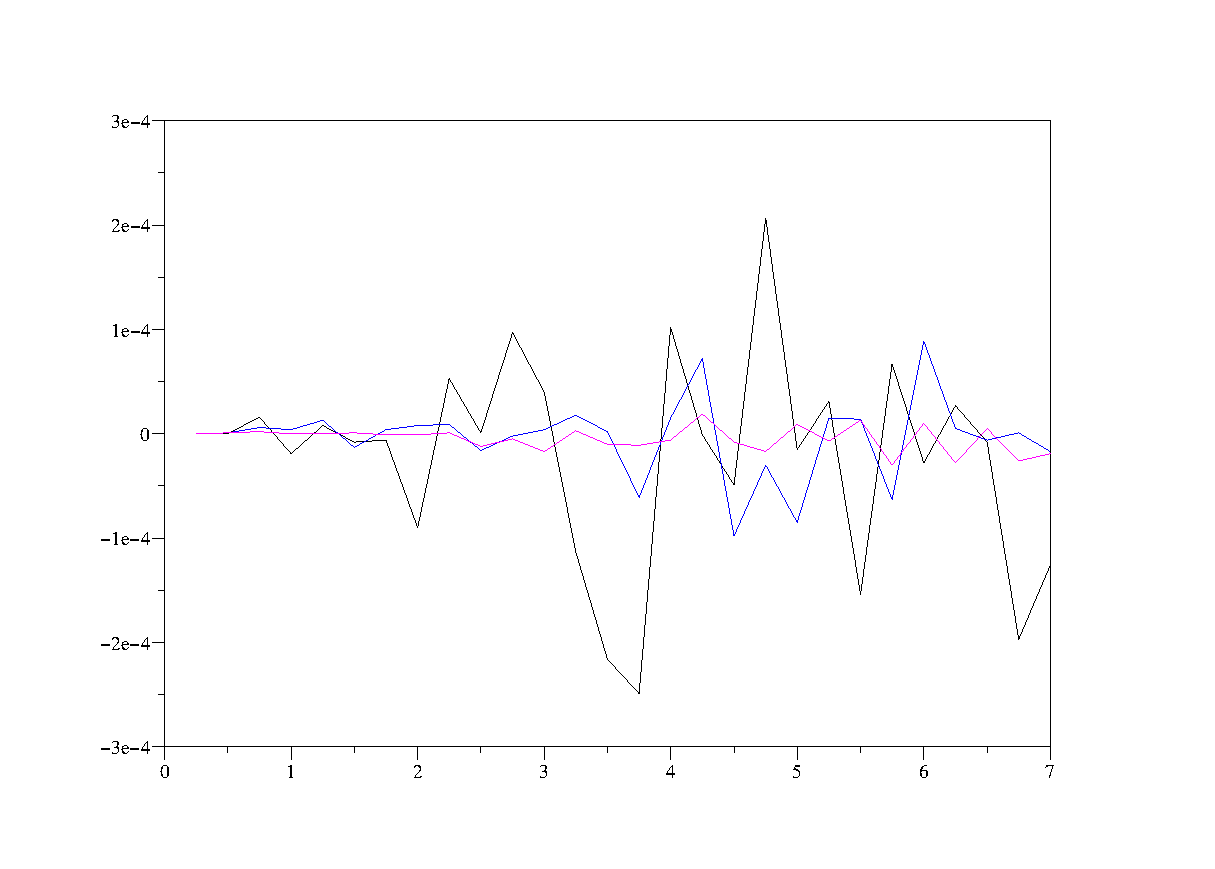
\includegraphics[height=8cm]{./figures/bondserrorY.eps}
\caption{Cumputation bonds error with martingale asset Y for $10 000$, $100 000$ and $1 000 000$ Monte-carlo
  draws, for $\tau=0.25$ and $M=28$ (Number of factor=$1$, $\gamma_i=0.15$ and $L(0,T_i,T_i)=0.05$).}
\label{bonderrorY}
\end{center}
\end{figure}
\begin{figure}[H]
\begin{center}
\includegraphics[height=8cm]{./figures/swptX.eps}
\caption{Swaption prices w.r.t. the time maturity  expiring at $T=7$
  computed with $100 000$ Monte-Carlo draws  with martingale asset X.} 
\label{swptX}
\end{center}
\end{figure}
\begin{figure}[H]
\begin{center}
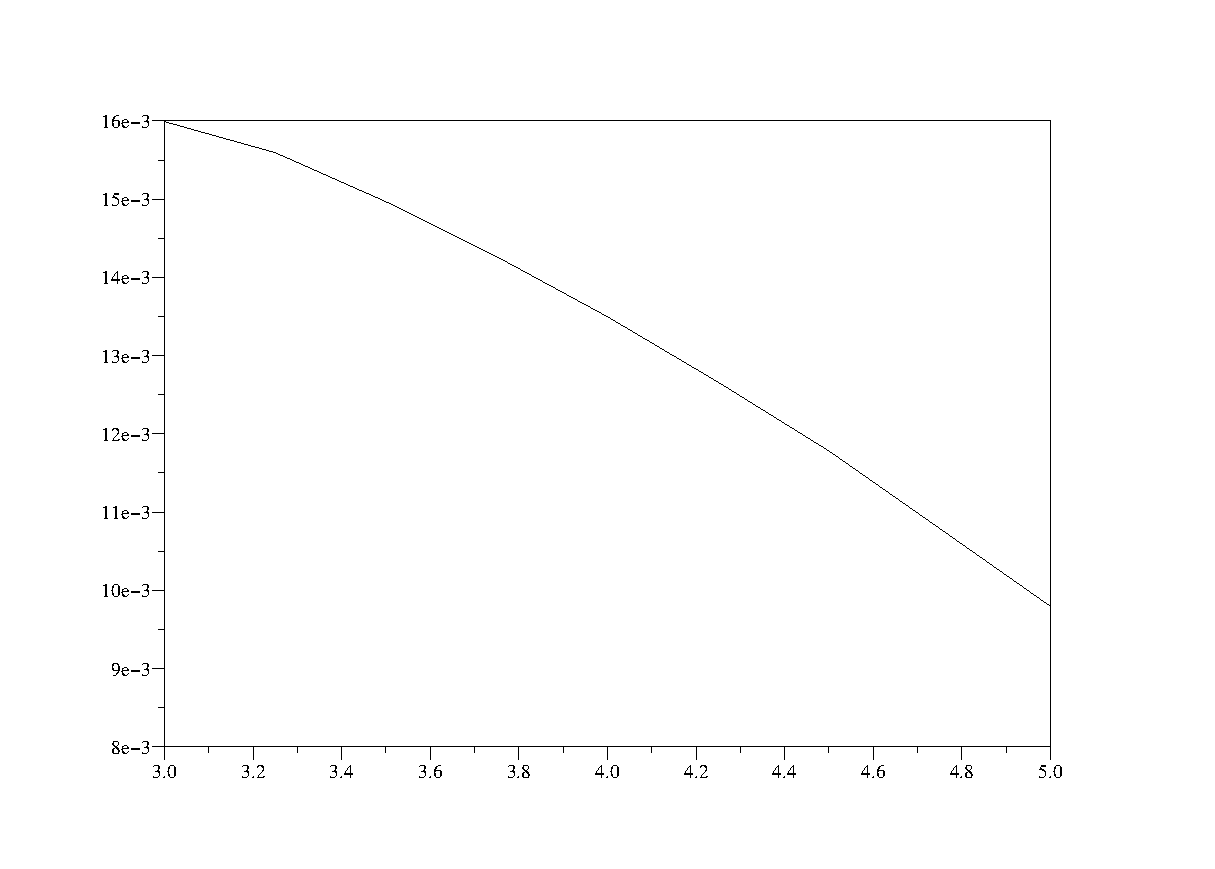
\includegraphics[height=8cm]{./figures/swptY.eps}
\caption{Swaption prices w.r.t. the time maturity  expiring at $T=7$
  computed with $100 000$ Monte-Carlo draws  with martingale asset Y.} 
\label{swptY}
\end{center}
\end{figure}
We can see that the swaption prices simulated with the asset $X$ and the asset $Y$
(for $\tau=0.25$ and $M=28$ Number of factor=$1$, $\gamma_i=0.15$ and
$L(0,T_i,T_i)=0.05$) are very similar with a relative precision of $10^{-2}$.


\subsection{Programming interface}


\subsubsection{C API of the pricer}

Functions name: 
\small{
\begin{verbatim}
int  lmm_caplet_terminalX_pricer(caplets, maturities, numMat, nb_MC, nb_factors, 
                                                           nb_time_step, strike, tenor)

int  lmm_swaption_payer_terminalX_pricer(&swaption_price, swaption_maturity, swap_maturity, 
					          nb_MC, nb_factors, nb_time_step, strike, tenor)

int  lmm_caplet_spotV_pricer( caplets ,  maturities , numMat , nb_MC , nb_factors , 
			                                  nb_time_step , strike ,  tenor);

int lmm_swaption_payer_spotV_pricer(&swaption_price ,  swaption_maturity , swap_maturity   , 
	               			  nb_MC ,  nb_factors ,  nb_time_step ,  strike , tenor);
\end{verbatim}
}

Arguments description:
\begin{itemize}
\item $tenor$ is the period in years of the rate (usually 3 or 6 months); type:double 
\item $numFac$ is the number of factors max 2; type: int
\item $swaption\_maturity$ is the swaption maturity in years; type: double
\item $swap\_maturity$ is the swap maturity in years ; type: double 
\item $strike$ strike of the option; type:double
\item $nb\_MC$ number of monte carlo paths; type: int
\item $nb\_factors$ is the number of factors max 2; type: int
\item $nb\_time\_step$ number of time steps in the euler scheme; type:int 
\end{itemize}


\subsubsection{calling the MartingaleX pricer from a C program}

\small{

\begin{verbatim}
/*************************************************************************************
 *
 *
 *
 *   Example: using Martingale X approach to price caplets and swaptions
 *          
 *
 *  
 *
 *************************************************************************************/
#include<stdio.h>

#include"lmm_martingaleX.h"

int main()
{
  
  double  tenor=0.5;   // period (in years) of the rate usually 3 or 6 months
  int numMat;     
  double *caplets;
  int i;
  double* maturities;
  double swaption_price;
  double swaption_maturity=3;  // swaption maturity in years
  double swap_maturity=7.;     // swap maturity in years
  int nb_MC   =10000;          // number of monte carlo paths
  int nb_time_step=10;         // number of time steps in the euler scheme
  double  strike=0.05;         // strike 
  int nb_factors=2;            // number of factors
  
  
  numMat=(int)(swap_maturity/tenor);
  caplets=(double*)malloc(numMat*sizeof(double));
  maturities=(double*)malloc(numMat*sizeof(double));

  lmm_caplet_terminalX_pricer(caplets, maturities, numMat, nb_MC, nb_factors, 
			      nb_time_step, strike, tenor);
  lmm_swaption_payer_terminalX_pricer(&swaption_price, swaption_maturity, swap_maturity, 
			      nb_MC, nb_factors, nb_time_step, strike, tenor);
  
  for(i=1;i<numMat;i++)
    {
      printf("Caplet(Ti=%lf,%lf,K=%lf)=%lf \n",tenor*i,tenor*i + tenor , strike , caplets[i]);
    }
	
  printf("Swaption price:\n");
  printf("Spt(T=%lf,%lf,K=%lf)=%lf \n",swaption_maturity, swap_maturity, strike, swaption_price);
	
  free(caplets);
  free(maturities);

  return(1);
}


\end{verbatim}

}



we obtain the following result:

\small{

\begin{verbatim}
$ lmm_martingaleX_example 
Caplet prices:
Caplet(Ti=0.500000,1.000000,K=0.050000)=0.003621 
Caplet(Ti=1.000000,1.500000,K=0.050000)=0.004856 
Caplet(Ti=1.500000,2.000000,K=0.050000)=0.005758 
Caplet(Ti=2.000000,2.500000,K=0.050000)=0.006413 
Caplet(Ti=2.500000,3.000000,K=0.050000)=0.006968 
Caplet(Ti=3.000000,3.500000,K=0.050000)=0.007332 
Caplet(Ti=3.500000,4.000000,K=0.050000)=0.007569 
Caplet(Ti=4.000000,4.500000,K=0.050000)=0.007861 
Caplet(Ti=4.500000,5.000000,K=0.050000)=0.008020 
Caplet(Ti=5.000000,5.500000,K=0.050000)=0.008182 
Caplet(Ti=5.500000,6.000000,K=0.050000)=0.008337 
Caplet(Ti=6.000000,6.500000,K=0.050000)=0.008330 
Caplet(Ti=6.500000,7.000000,K=0.050000)=0.008264 
Swaption price:
Spt(T=3.000000,7.000000,K=0.050000)=0.025182 
$ 
\end{verbatim}
}


\subsubsection{calling the MartingaleV pricer from a C program}

\small{

\begin{verbatim}
/**********************************************************************************************
 *
 *
 *
 *   Example: using Martingale V approach to price caplets and swaptions
 *
 *
 *
 *
 *********************************************************************************************/
#include<stdio.h>

#include"lmm_martingaleV.h"


int main()
{


  double  tenor=0.5;   // period (in years) of the rate usually 3 or 6 months
  int numMat;     
  double *caplets;
  int i;
  double* maturities;
  double swaption_price;
  double swaption_maturity=3;  // swaption maturity in years
  double swap_maturity=7.;     // swap maturity in years
  int nb_MC   =10000;          // number of monte carlo paths
  int nb_time_step=10;         // number of time steps in the euler scheme
  double  strike=0.05;         // strike 
  int nb_factors=2;            // number of factors

  
  
  numMat=(int)(swap_maturity/tenor);
  maturities=(double*)malloc((numMat+1)*sizeof(double));
  caplets=(double*)malloc((numMat+1)*sizeof(double));
  lmm_caplet_spotV_pricer( caplets ,  maturities , numMat , nb_MC , nb_factors , 
			   nb_time_step , strike ,  tenor);
  lmm_swaption_payer_spotV_pricer(&swaption_price ,  swaption_maturity , swap_maturity   , 
				  nb_MC ,  nb_factors ,  nb_time_step ,  strike , tenor);

  for(i=1;i<numMat;i++)
    {
      printf("Caplet(Ti=%lf,%lf,K=%lf)=%lf \n", tenor*i ,tenor*(i+1) , strike , caplets[i]);
    }
  printf("Spt(T=%lf,%lf,K=%lf)=%lf \n",swaption_maturity, swap_maturity, strike, swaption_price);
  free(caplets);
  free(maturities);

  return(1);
}

\end{verbatim}

}

we obtain the following result:

\small{

\begin{verbatim}
$ lmm_martingaleV_example 
Caplet(Ti=0.500000,1.000000,K=0.050000)=0.003631 
Caplet(Ti=1.000000,1.500000,K=0.050000)=0.004861 
Caplet(Ti=1.500000,2.000000,K=0.050000)=0.005767 
Caplet(Ti=2.000000,2.500000,K=0.050000)=0.006418 
Caplet(Ti=2.500000,3.000000,K=0.050000)=0.006967 
Caplet(Ti=3.000000,3.500000,K=0.050000)=0.007347 
Caplet(Ti=3.500000,4.000000,K=0.050000)=0.007592 
Caplet(Ti=4.000000,4.500000,K=0.050000)=0.007895 
Caplet(Ti=4.500000,5.000000,K=0.050000)=0.008064 
Caplet(Ti=5.000000,5.500000,K=0.050000)=0.008215 
Caplet(Ti=5.500000,6.000000,K=0.050000)=0.008379 
Caplet(Ti=6.000000,6.500000,K=0.050000)=0.008381 
Caplet(Ti=6.500000,7.000000,K=0.050000)=0.008326 
Spt(T=3.000000,7.000000,K=0.050000)=0.025197 
$ 
\end{verbatim}
}


\subsubsection{A Scilab function for the MartingaleX and MartingaleV pricers}

The scilab functions are given below:


\small{
\begin{verbatim}
lmm_cap_martX_sci(period , nb_fac , maturity , strike )
lmm_swpt_martX_sci(period , nb_fac , swpt_maturity , swp_maturity , strike )
lmm_cap_spotV_sci(period , nb_fac , maturity , strike )
lmm_swpt_spotV_sci(period , nb_fac , swpt_maturity , swp_maturity , strike )
\end{verbatim} 
}

they can be found in the file lmm\_scilab.sci,  they return the price of the options  and the input parameters are 

\begin{itemize}
\item {\it period} is the period length of the rate; type:double
\item {\it nb\_fac} is the number of factors; type: int
\item {\it maturity} is the maturity used to price all caplets; type: double
\item {\it swpt\_mat} is the swpation maturity in years; type: double
\item {\it swp\_mat} is th swap maturity in years; type: double
\item {\it strike} the strike; type: double
\end{itemize}


{\bf Loading the scilab functions}: first you should compile the library, report to the README file. At the scilab ``File'' menu click on ``File Operations'' then select the file ``lmm\_scilab.sci'' and click on ``Getf'' buttom, it will produce something like this in ``scilex''
\small{
\begin{verbatim} 
-->;getf("/home/der_mif/jose/recherche/taux/prog/cprog/bgmPremia/code/lmm_scilab.sci");
\end{verbatim} 
}

all functions within this file are now available at the prompt or can be called from a scilab program. 
 
We illustrate the use of the above functions: 

We obtained the following result from scilab-2.7:

\small{
\begin{verbatim}
-->b=lmm_cap_martX_sci(0.5 , 2 , 7 , 0.05)                                       
shared archive loaded
Link done
 b  =
 
!   0.           0.  !
!   0.0036211    0.5 !
!   0.0048560    1.  !
!   0.0057583    1.5 !
!   0.0064130    2.  !
!   0.0069682    2.5 !
!   0.0073320    3.  !
!   0.0075693    3.5 !
!   0.0078611    4.  !
!   0.0080204    4.5 !
!   0.0081819    5.  !
!   0.0083375    5.5 !
!   0.0083296    6.  !
!   0.0082636    6.5 !
 
-->
\end{verbatim} 
}

\small{
\begin{verbatim}
 
-->b=lmm_swpt_martX_sci(0.5,2,3,7,0.05)
shared archive loaded
Link done
 b  =
 
    0.0251820  
 
-->
\end{verbatim} 
}


\small{
\begin{verbatim}

-->b=lmm_swpt_spotV_sci(0.5,2,3,7,0.05)
shared archive loaded
Link done
 b  =
 
    0.0251971   
-->
\end{verbatim} 
}

The $lmm_cap_spotV_sci$ function leads to failure of the scilab program, we suggest not to use it. 





 
%\begin{thebibliography}{1}


\begin{thebibliography}{1}

\bibitem{brace1} A. Brace, ``Rank 2 swaption formulae''. Working praper.
 
\bibitem{braceGatarekMusiela} A. Brace, D. Gatarek, M. Musiela, ``The market model of interest rate dynamics'', {\it Mathematical finance}, 7, 127-155.

\bibitem{CLProtter} E.Cl\'ement, D. Lamberton, P.Protter, ``An Analysis of a Least Squares Regression Algorithm for American Option Pricing'', {\it Finance and Stochastic},\textbf{17}, pp. 448-471, 2002

\bibitem{collinDufresneGoldstein} P. Collin Dufresne, R. S. Goldstein, ``Generalizing the affine framework to HJM and random field models'', Working paper.

\bibitem{carrMadan} P. Carr, D. B., Madan, ``Option valuation using fast Fourier tansform'', {\it Journal of Computational Finance}, Vol 2, N$^0$ 4, 61-73, 333.


\bibitem{freeGZ} P. Glasserman and X. Zhao, ``Arbitrage-free discretization of lognormal forward Libor and swap rate models'', {\it Finance and Stochastics} (2000).

\bibitem{LambLap} D. Lamberton, B. Lapeyre, ``Introduction to Stochastic Calculus Applied to Finance'', CRC Press, 1996

\bibitem{Pedersen99} M. B. Pedersen, ``Bermudan Swaptions in the LIBOR Market Model'', {\it SimCorp Financial Research Working Paper}, 1999

\bibitem{Pelsser03} R. Pietersz, A. Pelsser, M. van Regenmortel, ``Fast Drift Approximated Pricing in the BGM Model'', {\emph SSRN Working Paper}, 2004

\bibitem{wuzhang} L. Wu, F. Zhang, ``Libor Market Model : from deterministic to stochastic volatility'', Working paper, 2002




\end{thebibliography}




\input premiaend

\end{document}
